\documentclass[12pt,twoside,a4paper]{report}

% Select encoding of your inputs
\usepackage[utf8]{inputenc}

% Make latex understand and use the typographic
% rules of the language used in the document.
\usepackage[english]{babel}

% Use the vector font Latin Modern which is going
% to be the default font in latex in the future.
\usepackage{lmodern}

% Choose the font encoding
\usepackage[T1]{fontenc}

% Use color in tables
\usepackage[table]{xcolor}
\usepackage{array}
\usepackage{multirow}

% Load a colour package
\usepackage{xcolor}
\definecolor{aaublue}{RGB}{33,26,82}  %<--define aaublue
\definecolor{white}{RGB}{255,255,255} %<--define white

% The standard graphics inclusion package
\usepackage{graphicx}

\makeatletter
  \g@addto@macro\@floatboxreset\centering %<--centering all figures
\makeatother

\usepackage{adjustbox}

% Set up how figure and table captions are displayed
\usepackage{float}
\usepackage{caption}
\usepackage{subcaption}
\captionsetup
{
  justification = centering,    %<--centering caption with multiple lines
  font          = footnotesize, %<--set font size to footnotesize
  labelfont     = bf,           %<--bold label (e.g., Figure 3.2) font
  belowskip     = -15pt
}
\captionsetup[subfigure]
{
  justification = centering, %<--centering subfigure caption text
  singlelinecheck=false,
  font = footnotesize        %<--font size for subfigures
} 

% Enable row combination in tables
\usepackage{multirow}

% Make space between table lines and text
\renewcommand{\arraystretch}{1.5}

% Enable commands like \st (strike out) and \hl (high light)
\usepackage{soul}

% Make the standard latex tables look so much better
\usepackage{array,booktabs}

% Enable the use of frames around, e.g., theorems
% The framed package is used in the example environment
\usepackage{framed}
\usepackage{colortbl}
\usepackage{longtable}
\usepackage{xcolor}
\usepackage{textcomp}

%-------MATHEMATICS---------------------------------
% Defines new environments such as equation,
% align and split 
\usepackage{amsmath}
\usepackage{relsize}
% Adds new math symbols
\usepackage{amssymb}
% Use theorems in your document
% The ntheorem package is also used for the example environment
% When using thmmarks, amsmath must be an option as well. Otherwise \eqref doesn't work anymore.
\usepackage[framed,amsmath,thmmarks]{ntheorem}
\usepackage{xifthen}%<--enables ifthenelse which is used in macros

\usepackage{siunitx} 
\sisetup{decimalsymbol=period}%<--\num{} will swich commas with periods
\sisetup{detect-weight}
%---------------------------------------------------

%-------PAGE LAYOUT---------------------------------
% Change margins, papersize, etc of the document
\usepackage[
  left=25mm,% left margin on an odd page %tidligere 25mm for baade right og left
  right=25mm,% right margin on an odd page
  top=35mm,
  ]{geometry}
  
% Modify how \chapter, \section, etc. look
% The titlesec package is very configureable
\usepackage{titlesec}
\makeatletter
\def\ttl@mkchap@i#1#2#3#4#5#6#7{%
    \ttl@assign\@tempskipa#3\relax\beforetitleunit
    \vspace{\@tempskipa}%<<<<<< REMOVE THE * AFTER \vspace
    \global\@afterindenttrue
    \ifcase#5 \global\@afterindentfalse\fi
    \ttl@assign\@tempskipb#4\relax\aftertitleunit
    \ttl@topmode{\@tempskipb}{%
        \ttl@select{#6}{#1}{#2}{#7}}%
    \ttl@finmarks  % Outside the box!
    \@ifundefined{ttlp@#6}{}{\ttlp@write{#6}}}
\makeatother

\titlespacing{\chapter}{0pt}{0pt}{10pt}
\titlespacing{\section}{0pt}{0pt}{-5pt}
\titlespacing{\subsection}{0pt}{8pt}{-5pt}
\titlespacing{\subsubsection}{0pt}{6pt}{-10pt}

\titleformat*{\section}{\normalfont\Large\bfseries\color{aaublue}}
\titleformat*{\subsection}{\normalfont\large\bfseries\color{aaublue}}
\titleformat*{\subsubsection}{\normalfont\normalsize\bfseries\color{aaublue}}

\usepackage{titlesec, blindtext, color}
%\color{gray75}{gray}{0.75}
\newcommand{\hsp}{\hspace{20pt}}
\titleformat{\chapter}[hang]{\Huge\bfseries}{\thechapter\hsp\textcolor{aaublue}{|}\hsp}{0pt}{\Huge\bfseries}

% Change the headers and footers
\usepackage{fancyhdr}
\setlength{\headheight}{15pt}
\pagestyle{fancy}
\fancyhf{} %delete everything
\renewcommand{\headrulewidth}{0pt} %remove the horizontal line in the header
\fancyhead[RO,LE]{\color{aaublue}\small\nouppercase\leftmark} %even page - chapter title
\fancyhead[LO]{}
\fancyhead[RE]{} 
\fancyhead[CE]{}
\fancyhead[CO]{}
\fancyfoot[RE,LO]{\thepage}
\fancyfoot[LE,RO]{} %page number on all pages
\fancyfoot[CE,CO]{}

% change first page of all chapters header and footer to fancy style
\makeatletter
\let\ps@plain\ps@fancy
\makeatother

% Do not stretch the content of a page. Instead,
% insert white space at the bottom of the page
\raggedbottom

% Enable arithmetics with length. Useful when typesetting the layout.
\usepackage{calc}
%---------------------------------------------------

%-------BIBLIOGRAPHY--------------------------------
%setting references (using numbers) and supporting i.a. Chicargo-style:
\usepackage{etex}
\usepackage{etoolbox}
\usepackage{keyval}
\usepackage{ifthen}
\usepackage{url}
\usepackage{csquotes}
\usepackage[backend=biber, url=true, doi=true, style=numeric, sorting=none]{biblatex}
\addbibresource{setup/bibliography.bib}
%---------------------------------------------------

%-------MISC----------------------------------------
%%% Enables the use FiXme refferences. Syntax: \fxnote{...} %%%
\usepackage[footnote, draft, english, silent, nomargin]{fixme}
%With "final" instead of "draft" an error will ocure for every FiXme under compilation.

%%% allows use of lorem ipsum (generate i.e. pagagraph 1 to 5 with \lipsum[1-5]) %%%
\usepackage{lipsum}

%%% Enables figures with text wrapped tightly around it %%%
\usepackage{wrapfig}

%%% Enable use of dashed lines in tables ( \hdashline )
\usepackage{arydshln}

%%% Section debth included in table of contents (1 = down to sections) %%%
\setcounter{tocdepth}{1}

%%% Section debth for numbers (1 = down to sections) %%%
\setcounter{secnumdepth}{1}

\usepackage{tocloft}
\setlength{\cftbeforetoctitleskip}{0 cm}
\renewcommand{\cftpartpresnum}{Part~}
\let\cftoldpartfont\cftpartfont
\renewcommand{\cftpartfont}{\cftoldpartfont\cftpartpresnum}
%---------------------------------------------------

%-------HYPERLINKS----------------------------------
% Enable hyperlinks and insert info into the pdf
% file. Hypperref should be loaded as one of the 
% last packages
\usepackage{nameref}
\usepackage{hyperref}
\usepackage{bookmark}
\hypersetup{%
	%pdfpagelabels=true,%
	plainpages=false,%
	pdfauthor={Author(s)},%
	pdftitle={Title},%
	pdfsubject={Subject},%
	bookmarksnumbered=true,%
	colorlinks,%
	citecolor=aaublue,%
	filecolor=aaublue,%
	linkcolor=aaublue,% you should probably change this to black before printing
	urlcolor=aaublue,%
	pdfstartview=FitH%
}
%---------------------------------------------------

% remove all indentations
\setlength\parindent{0pt}
\parskip 5mm
\usepackage{verbatim}

\definecolor{Gra}{RGB}{230,230,230}

%creates a nice-looking C#-text
\newcommand{\CC}{C\nolinebreak\hspace{-.05em}\raisebox{.3ex}{\scriptsize\text \#} }

%enables multi column lists
\usepackage{multicol}

%enables code-examples
\usepackage{listings}

\definecolor{coolblue}{RGB}{32,95,128}
\definecolor{mygreen}{rgb}{0,0.6,0}
\definecolor{mygray}{rgb}{0.5,0.5,0.5}
\definecolor{mymauve}{rgb}{0.58,0,0.82}
\usepackage{textcomp}
\definecolor{listinggray}{gray}{0.9}
\definecolor{lbcolor}{rgb}{0.9,0.9,0.9}

%for c code
\lstdefinestyle{cstyle}{
  backgroundcolor=\color{lbcolor},
	tabsize=4,
	rulecolor=,
	language=C,
  basicstyle=\scriptsize,
  upquote=true,
  aboveskip={1.5\baselineskip},
  columns=fixed,
  showstringspaces=false,
  extendedchars=true,
  breaklines=true,
  prebreak = \raisebox{0ex}[0ex][0ex]{\ensuremath{\hookleftarrow}},
  frame=single,
  showtabs=false,
  numbers=left,
  captionpos=b,
  numbersep=5pt,
  numberstyle=\tiny\color{mygray},
  showspaces=false,
  showstringspaces=false,
  identifierstyle=\ttfamily,
  keywordstyle=\color[rgb]{0,0,1},
  commentstyle=\color[rgb]{0.133,0.545,0.133},
  stringstyle=\color[rgb]{0.627,0.126,0.941},
}
%for python code
\lstdefinestyle{pythonstyle}{
    backgroundcolor=\color{lbcolor},
    tabsize=4,
    rulecolor=,
    language=python,
    basicstyle=\scriptsize,
    upquote=true,
    aboveskip={1.5\baselineskip},
    columns=fixed,
    showstringspaces=false,
    extendedchars=true,
    breaklines=true,
    prebreak = \raisebox{0ex}[0ex][0ex]{\ensuremath{\hookleftarrow}},
    frame=single,
    showtabs=false,
    numbers=left,
    captionpos=b,
    numbersep=5pt,
    numberstyle=\tiny\color{mygray},
    showspaces=false,
    showstringspaces=false,
    identifierstyle=\ttfamily,
    keywordstyle=\color[rgb]{0,0,1},
    commentstyle=\color[rgb]{0.133,0.545,0.133},
    stringstyle=\color[rgb]{0.627,0.126,0.941},
}
%for matlab code
\lstdefinestyle{matlabstyle}{
    backgroundcolor=\color{lbcolor},
    tabsize=4,
    rulecolor=,
    language=Matlab,
    basicstyle=\scriptsize,
    upquote=true,
    aboveskip={1.5\baselineskip},
    columns=fixed,
    showstringspaces=false,
    extendedchars=true,
    breaklines=true,
    prebreak = \raisebox{0ex}[0ex][0ex]{\ensuremath{\hookleftarrow}},
    frame=single,
    showtabs=false,
    numbers=left,
    captionpos=b,
    numbersep=5pt,
    numberstyle=\tiny\color{mygray},
    showspaces=false,
    showstringspaces=false,
    identifierstyle=\ttfamily,
    keywordstyle=\color[rgb]{0,0,1},
    commentstyle=\color[rgb]{0.133,0.545,0.133},
    stringstyle=\color[rgb]{0.627,0.126,0.941},   
}
%for inline c, syntax: \cline{ codeHere(); }
\lstdefinestyle{cinline}{
    style=cstyle,
    basicstyle=\small,
}
\newcommand\inlinec[1]{ \lstinline[style=cinline]{#1} }

%for inline python, syntax: \pythonline{ codeHere(); }
\lstdefinestyle{pythoninline}{
    style=pythonstyle,
    basicstyle=\small,
}
\newcommand\inlinepython[1]{ \lstinline[style=pythoninline]{#1} }

%for inline matlab, syntax: \matlabline{ codeHere(); }
\lstdefinestyle{matlabinline}{
    style=matlabstyle,
    basicstyle=\small,
}
\newcommand\inlinematlab[1]{ \lstinline[style=matlabinline]{#1} }

\usepackage{enumitem}
%\usepackage[citestyle=authoryear,natbib=true]{biblatex}

% Figures - TIKZ
\usepackage{tikz}
\usepackage[americanresistors,americaninductors,americancurrents, americanvoltages]{circuitikz}

% Wall of text logo
\newcommand{\walloftextalert}[0]{\includegraphics[width=\textwidth]{walloftext.png}}

\usepackage{pdfpages}
\usepackage{lastpage}
\usepackage{epstopdf}

\setlength{\headheight}{21pt}

\hfuzz=\maxdimen
\tolerance = 10000
\hbadness  = 10000

\usepackage{siunitx}
\graphicspath{{./figures/}}
% package inclusion and set up of the document

%Macro for 'where'-enviroment was improved by Andrea and Niels :-)

%-----------UNITS-------------------------------------------
\newcommand{\unit}[1]{&& \left[\si{#1}\right]}
%
%\newcommand{\unit}[1]{[\si{#1}]}            %<<| Use these if you want equations to be
%\newcommand{\eq}[2]{&&\si{#1} &= \si{#2}&&} %<<| centered.. .. will appear scrambled
%                                            %  | from one equation to the next though..
%                                            %  | and does not work with long equations.. :/
%
%-----------------------------------------------------------

%-----------WHERE ENVIRONMENT-------------------------------
\newenvironment{where}{\leavevmode{\parindent=1em\indent} Where:\\}{}
\newcommand{\va}[3]
{
  \begin{tabular}{p{20pt} p{40pt} p{290pt} l}
    & { $#1$ } & { #2 } & \ifthenelse{\isempty{ #3 }}  {}  {[{\si{#3}}]} \\
  \end{tabular}\\
}
%-----------------------------------------------------------

%-----------TikZ SETTINGS-----------------------------------
\tikzset{
  block/.style    = {draw, thick, rectangle,
                     minimum height = 2.1em,
                     minimum width = 1.7em},
  sum/.style      = {draw, circle, inner sep=3pt} %<--Adder
}
%-----------------------------------------------------------

%------------VECTORS----------------------------------------
\renewcommand{\vec}[1]{\boldsymbol{\mathbf{#1}}}% my new macros

\begin{document}
%%% Prereport %%%
\setlength\cftaftertoctitleskip{2pt}
\setlength\cftafterloftitleskip{6pt}
\setlength\cftafterlottitleskip{6pt}
\selectlanguage{english}
%\title{Cubli}

%%% Frontmatter Settings %%%
\pagestyle{empty} %disable headers and footers
\pagenumbering{roman} %use roman page numbering in the frontmatter I II...
\fancyfoot[RE,LO]{} %page number on all pages
\fancyfoot[LE,RO]{\thepage}
\fancyhead[LE,LO,RE,RO]{}

%%% Introductory Formalities %%%
%
\includepdf[pages={1}]{formalities/frontpage.pdf}
\pdfbookmark[0]{Front Page}{label:forside}%
\begin{titlepage}
  \addtolength{\hoffset}{0.5\evensidemargin-0.5\oddsidemargin} %set equal margins on the frontpage - remove this line if you want default margins
  \noindent%
  \begin{tabular}{@{}p{\textwidth}@{}}
    \toprule[2pt]
    \midrule
    \vspace{0.2cm}
    \begin{center}
    \Huge{\textbf{
      Autonomous Lawn Mower % insert your title here
    }}
    \end{center}
    \begin{center}
      \Large{
      Utilizing a Local Positioning System
      }
    \end{center}
    \vspace{0.2cm}\\
    \midrule
    \toprule[2pt]
  \end{tabular}
   \vspace{0.55 cm}
  \begin{figure}[!ht]
\centering
\includegraphics[width=0.8\textwidth]{figures/frontPageImage.pdf}
\label{fig:forside}
\end{figure}
  \vspace{-0.35 cm}
  \begin{center}
    {\large
      5. Semester Project Report %Insert document type (e.g., Project Report)
    }\\
    \vspace{0.2cm}
    {\Large
      Group 15gr510%Insert your group name or real names here
    }
  \end{center}
  \begin{center}
  Aalborg University\\
  Electronic Engineering \& IT\\
  Fredrik Bajers Vej 7\\
  DK-9220 Aalborg
  \end{center}
\end{titlepage}

\clearpage
\pagestyle{fancy}
%{\small
%\strut\vfill % push the content to the bottom of the page
%\noindent Copyright \copyright{} Aalborg University 2015\par
%\vspace{0.2cm}

%\noindent This report is compiled in \LaTeX, originally developed by Leslie Lamport, based on Donald Knuth's \TeX. The main text is written in \emph{Latin Modern} pt 12, designed by Bogusław Jackowski and Janusz M. Nowacki. 
%The document is compiled via the website \url{www.overleaf.com}, an online collaborative based \LaTeX-editor with instant preview, which enables multiple persons to edit the document simultaneously.
%Flowcharts and diagrams are made using Microsoft Visio. 
\clearpage
%\begin{document} 
\thispagestyle{empty}
\begin{titlepage}
\begin{nopagebreak}
{\samepage 

\begin{tabular}{r}
\hspace{-.6cm} \parbox{\textwidth}{  \raisebox{-5mm}{
  {
    
\includegraphics[width=.21\textwidth]{aaulogo-en}
  }
  \hspace{10pt}
  {
    
\includegraphics[width=.11\textwidth]{ntnulogo}
  }
}
\hspace{1.25cm} \parbox{8cm}{\begin{tabular}{l} %4.90
{\small \textbf{\textcolor{aaublue}{\colorbox{white}{9\textsuperscript{th} Semester}}}}\\
{\small \textbf{\textcolor{aaublue}{School of Information and}}}\\
{\small \textbf{\textcolor{aaublue}{Communication Technologies}}}\\ 
{\small \textbf{\textcolor{aaublue}{Electronics and IT}}}\\
{\small \textcolor{aaublue}{Fredrik Bajers Vej 7C}} \\
{\small \textcolor{aaublue}{9220 Aalborg}} \\
{\small \textcolor{aaublue}{\emph{http://www.sict.aau.dk/electronics-and-it}}}
\end{tabular}}}
\end{tabular}

\begin{tabular}{cc}
\parbox{7cm}{

\textbf{Title:}

Trajectory Planning for Cart Pendulum System\\

\textbf{Theme:}

\small{
Control Engineering\\
}


\parbox{8cm}{


\textbf{Project Period:}\\
Autumn 2017\\
21/08/2017 - 21/12/2017\\

\textbf{Participants:}\\
Niels Skov Vestergaard\\

\textbf{Supervisor:}\\
Anton Shiriaev\\
John-Josef Leth\\
}\\

\textbf{Pages:}\\

%\textbf{Appendices:}\\
%
\textbf{Concluded:} 21/12/2017\\

\vfill } &
\parbox{7cm}{
  \vspace{.15cm}
  \hfill
  \begin{tabular}{l}
  {\textbf{Synopsis}}\bigskip \\
  \fbox{
    \parbox{6.5cm}{\bigskip
     {\vfill{\small The aim of the project was to investigate a method for trajectory planning for a cart pendulum. To find an interesting trajectory, a task was posed for the system to complete.\\
The system was modeled and a simulation of the system dynamics created using MATLAB Simulink. To aid in the progress and to be able to show the result in a visual manner a graphical layer was added to the simulation.\\
The properties of the system was assessed using phase portraits. It was found that the phase portrait can be altered making different trajectories possible by designing the input force as a solution to the integral of the system dynamics given some initial conditions and constraints.
     \bigskip}}
     }}
   \end{tabular}}
\end{tabular}} \vspace{1cm}

%\textit{\phantom{A}Publication of this report's contents (including citation) without permission\\ \phantom{A}from the authors is prohibited.}\\

\end{nopagebreak}
\end{titlepage}
%\end{document}
%%% Preface %%%
%\cleardoublepage
%%%%%%%%%%%%%%%%%%%%%%%%%%%%%%%%%%%%%%%%%%%%%%%%5\chapter*{Preface}
\vspace{-12 pt}
\lipsum[3]\fxnote{Write prephase}

\textbf{Reading Instructions}
\vspace{-10 pt}
\begin{itemize}
\item[-] \lipsum[6]\fxnote{Write reading instructions}
\end{itemize}

%
\textbf{Text by:}\\
\vspace{-12 pt}
\begin{table}[H]
	\centering
		\begin{tabular}{c c c}
			&&\\
	    \multicolumn{3}{c}{\underline{\phantom{- Niels Skov Vestergaard -}}}\\
	    \multicolumn{3}{c}{Niels Skov Vestergaard}\\				
		\end{tabular}
\end{table}
\pagebreak

\pdfbookmark[0]{Table of Contents}{label: tableOfCentents}
\tableofcontents
\cleardoublepage


%%% Mainmatter Settings %%%
\pagenumbering{arabic} %use arabic page numbering in the mainmatter
\fancyfoot[RO,LE]{\thepage \text{ of} \pageref{LastPage}}
\fancyfoot[RE,LO]{}
\fancyhead[RE,LO]{}
\fancyhead[RE,LO]{\color{aaublue}\small\nouppercase\leftmark} %even page - chapter title
\pagestyle{fancy}


%---------- Chapter 1 ---------------------------------------- Problem Description
\chapter{Problem Description}\label{chap:problemDescription}

The system is underactuated, and nonlinear.

%The system in \autoref{fig:system}, is the well-known cart pendulum system. The system can only be controlled by a the force shown directly on the cart in the horisontal direction. So the system is underactuated, and nonlinear.

%\begin{figure}[H]
%  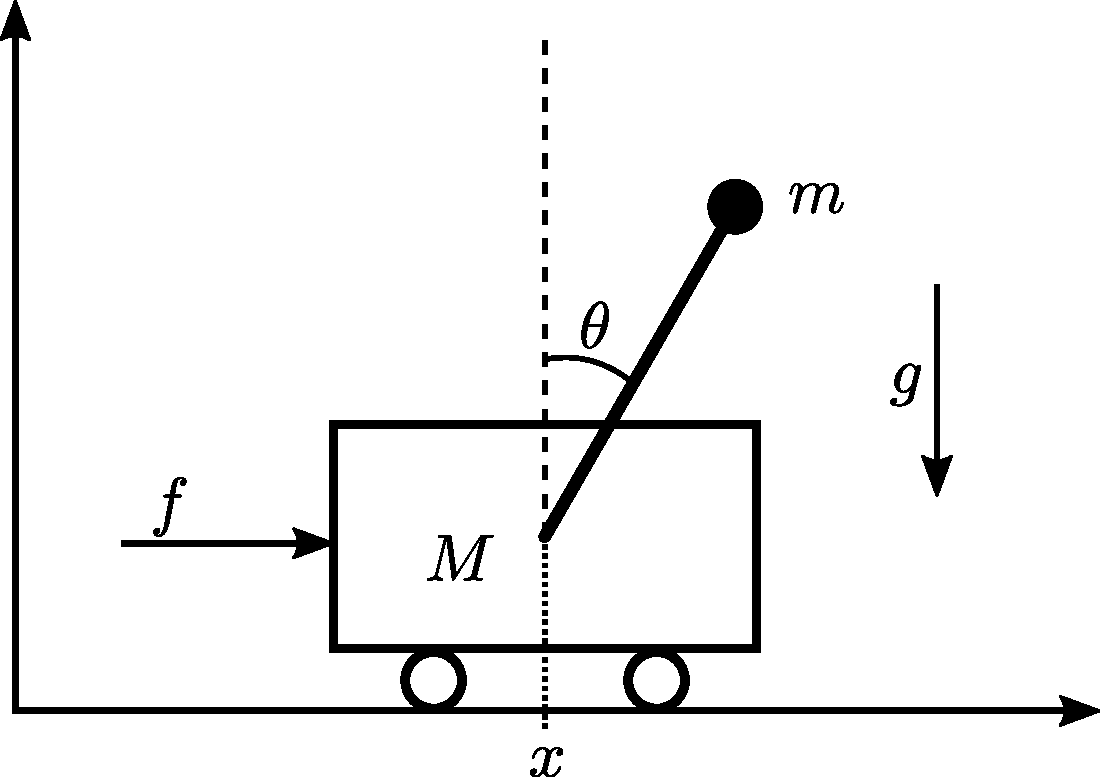
\includegraphics[width=.4\textwidth]{figures/system}
%  \caption{The cart pendulum system with generalized coordinates, $x$ and $\theta$, where $x$ is the center position of the cart, $\theta$ is the angle of the pendulum, $m$ is the point mass of the pendulum, $M$ is the mass of the cart, g is the gravitational acceleration and f is the force of actuation.}
%  \label{fig:system}
%\end{figure}

The system is presented with a specific task, see \autoref{fig:systemTask}. This aids in understanding the convinience of the presented trajectory planning tools, as the task requires nonlinear operation, where linearization alone is not enough.

\begin{figure}[H]
  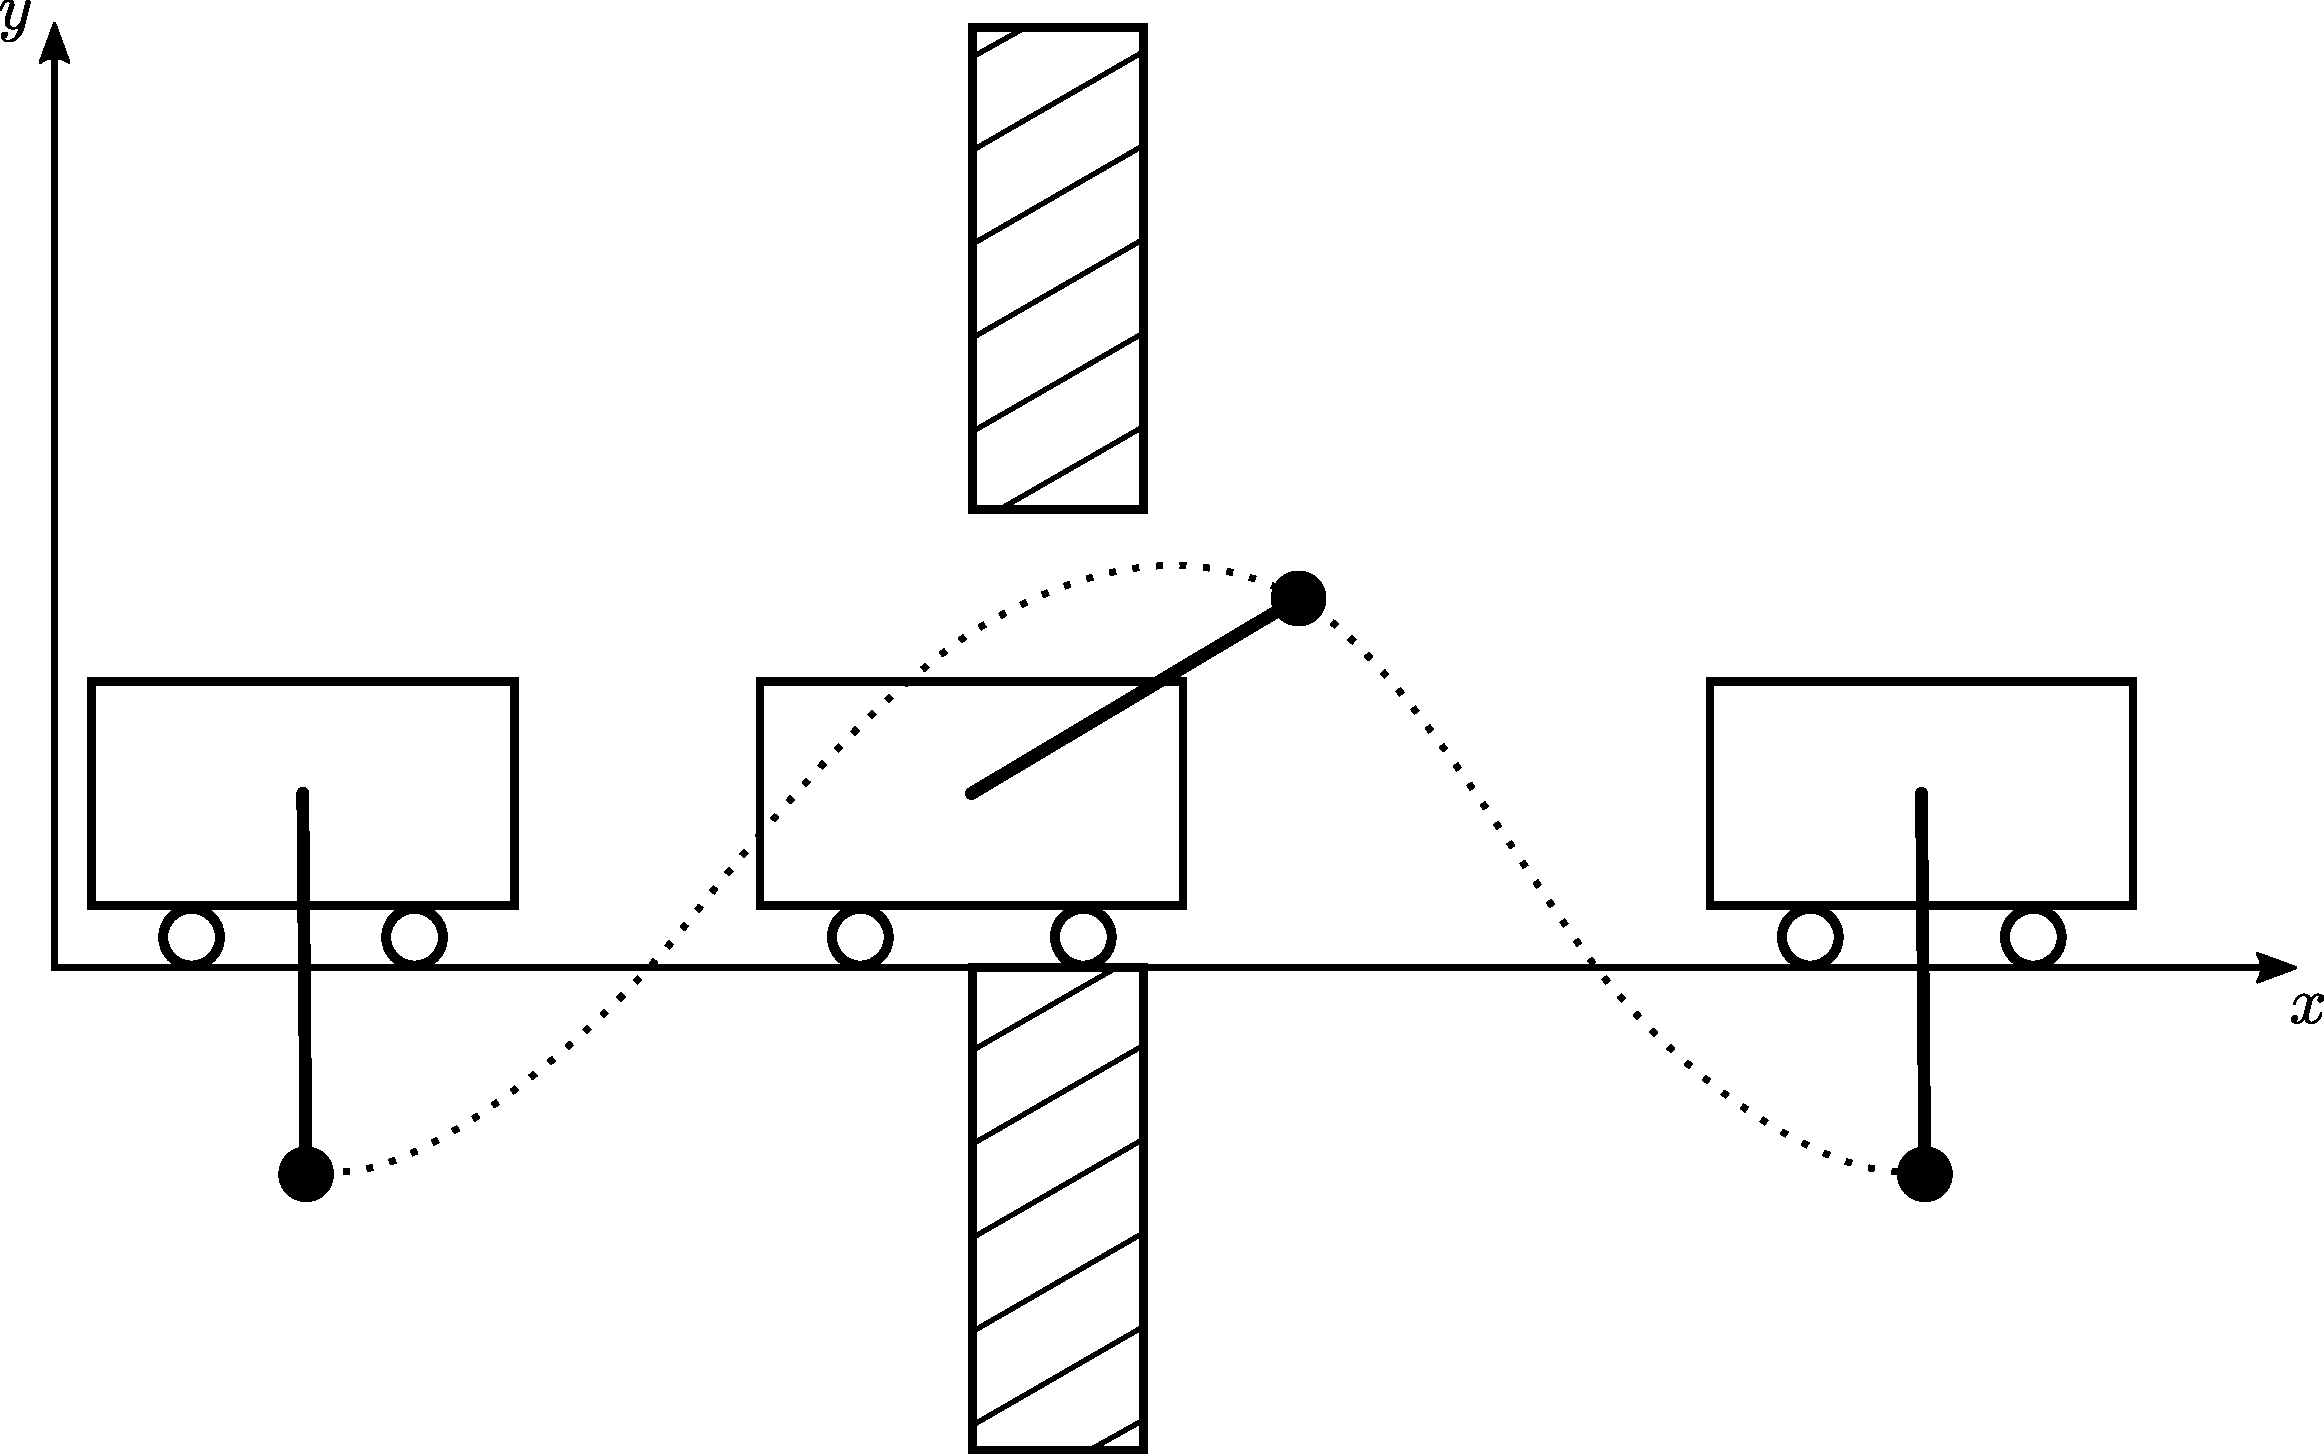
\includegraphics[width=.6\textwidth]{figures/systemTask}
  \caption{The task to be performed. The trajectory here is not realistic, and only shown to ilustrate the goal; avoiding the obstacles along the entire trajectory.}
  \label{fig:systemTask}
\end{figure}



%%% PART 1 %%%
\part{System and Stabilization}

%---------- Chapter 1 ---------------------------------------- Introduction
%\chapter{Introduction}

%---------- Chapter 2 ---------------------------------------- The System
\chapter{The System}
In this chapter, the system and the problem to be solved is presented. A model is developed along with a simulation presented here in form of a block diagram. Further the nonlinear nature of the system is investigated.

A system is provided by the automation and control department at Aalborg University (AAU). The setup is seen in \autoref{fig:systemSetup}, the parameters that can be measured directly are indicated.

\begin{figure}[H]
  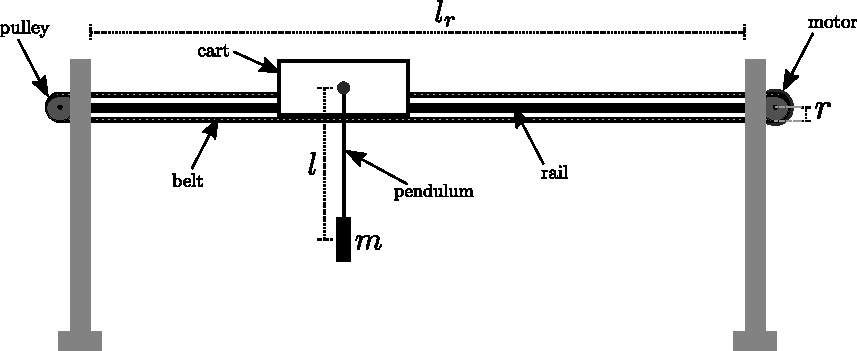
\includegraphics[width=.8\textwidth]{figures/systemSetup}
  \caption{The system setup provided by AAU, where $m$ is the mass of the pendulum weight attached at the end of the rod, $l$ is the length from pivot point to center of mass, $r$ is the radius of the pulley and $l_r$ is the effective length of the rail.}
  \label{fig:systemSetup}
\end{figure}

The mass of the cart cannot be directly measured as it is preferred not to take the system apart. This parameter is later estimated along with frictions in the system. \fxnote{streamline friction notation, see sources}

\begin{table}[H]
\begin{tabular}{|lp{.4cm}|l|l|l|}
  \hline %--------------------------------------------------------------------------------
  \textbf{Parameter}        &   & \textbf{Notation} & \textbf{Quantity} & \textbf{Unit} \\
  \hline %--------------------------------------------------------------------------------
  Pendulum Mass             &   &   $m$             &                   &               \\
  \hline %--------------------------------------------------------------------------------
  Cart Mass                 & * &   $M$             &                   &               \\
  \hline %--------------------------------------------------------------------------------
  Rod Length                &   &   $l$             &                   &               \\
  \hline %--------------------------------------------------------------------------------
  Pulley Radius             &   &   $r$             &                   &               \\
  \hline %--------------------------------------------------------------------------------
  Cart Coulomb Friction     & * &   $f_{c,c}$       &                   &               \\
  \hline %--------------------------------------------------------------------------------
  Cart Viscous Friction     & * &   $f_{c,v}$       &                   &               \\
  \hline %--------------------------------------------------------------------------------
  Pendulum Coulomb Friction & * &   $b_{p,c}$       &                   &               \\
  \hline %--------------------------------------------------------------------------------
  Pendulum Viscous Friction & * &   $b_{p,v}$       &                   &               \\
  \hline %--------------------------------------------------------------------------------
\end{tabular}
\caption{'*' indicates that the parameter is estimated.\label{table:systemParameters}}
\end{table}
%\section{Hardware}\label{sec:hardware}
%This section provides a brief overview of the hardware used in the cart pendulum setup.
\fxnote{add picture of the system (showing wires on cart)}
%
\section{Motors}\label{sec:motors}
There are two Maxon 370356 brushed DC motors, see \autoref{fig:maxonMotor}, used in the setup. \fxnote{source}.

% https://www.maxonmotor.com/maxon/view/product/motor/dcmotor/re/re50/370356
\fxnote{see url source in comment}

\begin{figure}[H]
  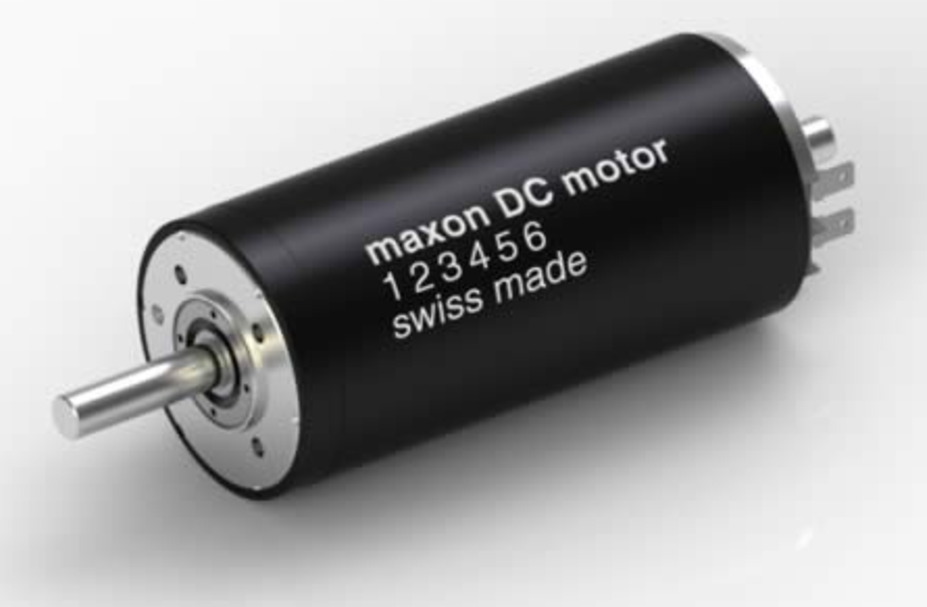
\includegraphics[width=.26\textwidth]{figures/maxonMotor}
  \caption{maxonMotor}
  \label{fig:maxonMotor}
\end{figure}

The most interesting characteristic of the maxon motor for the purposes of this report are shown in \autoref{table:motorParameters}.

\begin{table}[H]
  \begin{tabular}{|l|l|l|}
    \hline %--------------------------------------------------------------------------------------
    \textbf{Characteristic}                    & \textbf{Quantity} & \textbf{Unit}              \\
    \hline %--------------------------------------------------------------------------------------
    Nominal torque (max. continuous torque)    & \SI{420e-3}       &  \si{N \cdot m}            \\
    \hline %--------------------------------------------------------------------------------------
    Nominal current (max. continuous current)  & \SI{4.58}         &  \si{A}                    \\
    \hline %--------------------------------------------------------------------------------------
    Torque constant                            & \SI{93.4e-3}      &  \si{N\cdot m\cdot A^{-1}} \\
    \hline %--------------------------------------------------------------------------------------
    Rotor inertia                              & \SI{54.2e-6}      &  \si{kg\cdot m^2}          \\
    \hline %--------------------------------------------------------------------------------------
    Weight                                     & \SI{1.1}          &  \si{kg}                   \\
    \hline %--------------------------------------------------------------------------------------
  \end{tabular}
  \caption{'*' indicates that the parameter is estimated.\label{table:motorParameters}}
\end{table}

One of the motors is mounted on a pulley driving the belt, see \autoref{fig:systemSetup}. The other motor is disabled and acts only as a bearing at the pendulum pivot point.

\section{Motor Encoders}

Each of the two motors are equipped with an HEDS 5540 optical quadrature encoder, see \autoref{fig:maxonMotor}. The moment of inertia added by the encoder is negligibly small at only \SI{0.6e-6}{kg\cdot m^2} and is not mentioned further in this report.

%https://www.infineon.com/dgdl/Infineon-Encoder_HEDS-5540-A14-AP-v01_00-EN.pdf?fileId=5546d46147a9c2e40147d3d593970357
\fxnote{see url source in comment}

\begin{figure}[H]
  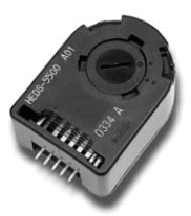
\includegraphics[width=.16\textwidth]{figures/infineonEncoderHEDS5540-A14}
  \caption{encoder}
  \label{fig:encoder}
\end{figure}

\section{Motor Controller}
Two Maxon ADS 50/10 motor controllers, see \autoref{fig:maxonMotorController}, are mounted on the cart pendulum setup. One on the side to control the driving motor and the other, not used in this project, mounted on the cart. The datasheet states that the motor controller weights \SI{0.38}{kg}, but again, since the remaining mass of the cart is unknown and can not be measured, the cart mass must be estimated.\fxnote{source}

% https://www.maxonmotor.com/maxon/view/product/control/Servoverstaerker-4-Q-DC/201583
\fxnote{see url source in comment}

\begin{figure}[H]
  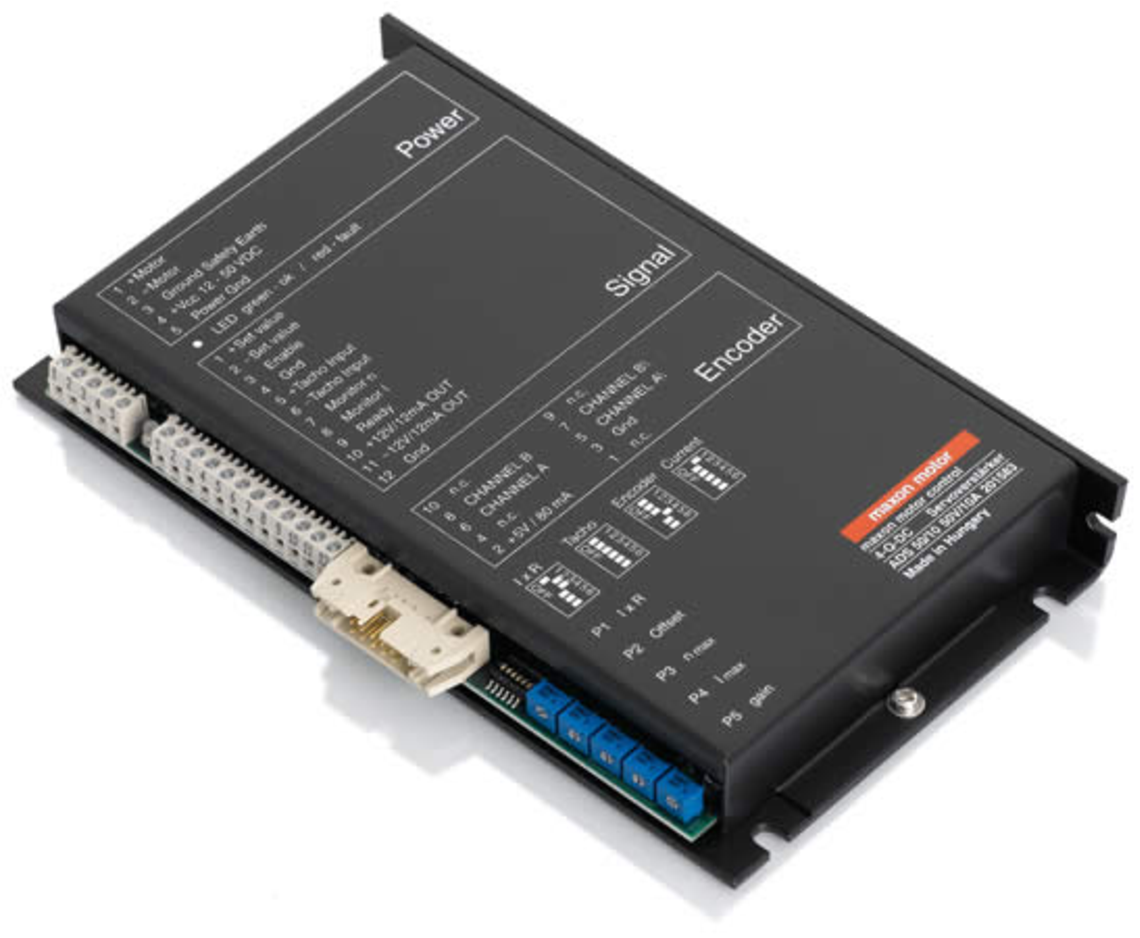
\includegraphics[width=.26\textwidth]{figures/maxonMotorController}
  \caption{maxonMotorController}
  \label{fig:maxonMotorController}
\end{figure}

The motor controller can be configured in four different modes,
\vspace{-10pt}
\begin{itemize}
  \item[-] Speed control using tacho signals
  \item[-] Speed control using encoder signals
  \item[-] IxR compensated speed control
  \item[-] Torque or current control
\end{itemize}
\vspace{-10pt}
The first three modes are forms of speed control while the last is current control relating directly to torque and thereby also force on the belt. The chosen mode for this project is therefore current control. The conversion from armature current to motor torque is by use of the torque constant given in \autoref{table:motorParameters}. To set the armature current the motor controller requires a $\pm$\SI{10}{V} input signal. This input is provided through a shield from the microcontroller, so the conversion to armature current is handled in the following.\fxnote{source}

\section{Micro Controller}
The control design is implemented on a Teensy 3.6 microcontroller, see \autoref{fig:teensy3_6}, provided in the setup. The armature current reference is provided through one of the microcontroller's two 12 bit DAC's (Digitl-to-Analog Converter) placed on an external pin of the microcontroller. The Teensy 3.6 runs on \SI{3.3}{V} provided by an onboard regulator from \SI{5}{V} USB supply, and so the analog output is in the range of $0-$\SI{3.3}{V} with a 12 bit resolution.\\
The motor encoders are decoded on the shield, see next section, and read through an 8 bit parallel data bus by the microcontroller.

\fxnote{source: https://www.sparkfun.com/products/14057}

\begin{figure}[H]
  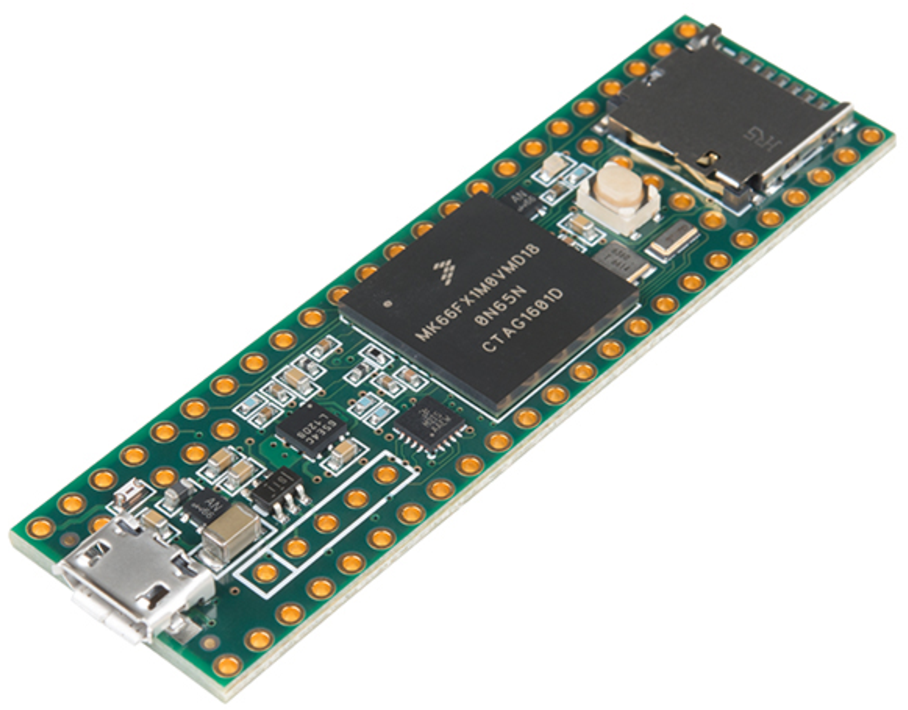
\includegraphics[width=.2\textwidth]{figures/teensy3_6}
  \caption{teensy3.6}
  \label{fig:teensy3_6}
\end{figure}

The Teensy 3.6 uses a bootloader which allows programming through USB using the Teensyduino add-on for the Arduino IDE.

\section{Shield}
A shield located by the microcontroller handles conversion/interfacing between the microcontroller and the setup. The motor encoders are decoded using Avago HCTL-2021-PLC decoders, mounted on the shield, which outputs 2000 ticks pr. revolution.\fxnote{source} This results in a resolution of $2\pi/2000=$ \SI{\pi e-3} rad/tic, for the pendulum angle, $\theta$, and $2\pi r /2000=\nolinebreak 2\pi\cdot 0.028 /2000\approx$ \SI{0.088e-3} m/tic for the position along $x$.
The armature current reference is provided from the microcontroller which as mentioned outputs $0-$\SI{3.3}{V} while the motor controller requires a $\pm$\SI{10}{V} input. This is handled by an amplification on the shield converting the $0-$\SI{3.3}{V} to the required $\pm$\SI{10}{V}.
A previous project group has tested the relation between armature current and different 12 bit values from the micro controller. The test was conducted using a current clamp and an oscilloscope to measure the armature current in the motor. By linear regression they arrived at the following relation,
%
\begin{flalign}
  \text{bit}_\text{DAC} &= 105.78 \cdot i_{a} + 1970  \ \ \ . & 
  \label{eq:Ia-bit}
\end{flalign}
%
An other way of measuring the current is from an output directly on the motor controller. It is found that this output is slightly different than the current measured directly over the motor using a current clamp. It is difficult to know if the torque constant supplied by the company is matched using one or the other way of measuring. So a test is conducted to verify \autoref{eq:Ia-bit}, in which the steady state hold force is measured directly on the cart using a luggage scale as an alternative Newton-meter. The results of the force test are seen in \autoref{fig:forceTest1} and \ref{fig:forceTest2} and a test journal is provided in \fxnote{refference appendix}.

\begin{figure}[H]
  \hspace{-10pt}
  \captionbox
  {
    forceTest1
    \label{fig:forceTest1}
  }
  {
    %\hspace{-1cm}
    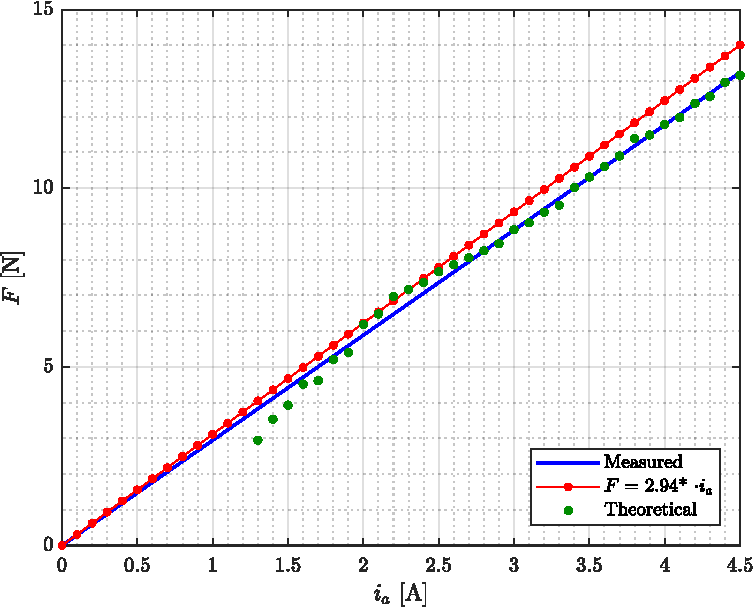
\includegraphics[width=.45\textwidth]{figures/forceTest1}%\vspace{-11pt}
  }
  \hspace{20pt}
  \captionbox 
  {
    forceTest2
    \label{fig:forceTest2}
  }
  {
    %\hspace{-1cm}
    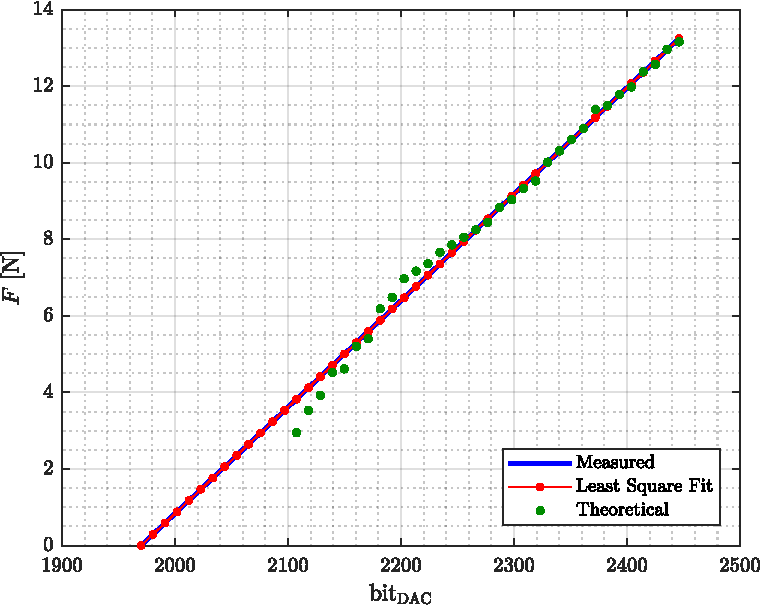
\includegraphics[width=.45\textwidth]{figures/forceTest2}\vspace{6pt}
  }  
\end{figure}

The measurements should be more correct at higher forces since friction then causes less disturbance in the measurements. However, no measurements are excluded in the regression as it is noted that the regression line fits the upper part of the data very well. Measurements lower than $F = 2.95$ were considered unreliable due to friction and therefore not included in the data-set.
In \autoref{fig:forceTest1} the armature current is scaled using \autoref{eq:Ia-bit} and the theoretical line is calculated using that $F = \tfrac{1}{r} k_\tau i_a$. As the theoretical line does not coincide exactly with the least square regression, \autoref{eq:Ia-bit} is tweaked so that,
\begin{flalign}
  \text{bit}_\text{DAC} &= 111.9 \cdot i_{a} + 1970  \ \ \ , & 
  \label{eq:Ia-bit-corrected}
\end{flalign}
which leads to the result seen in \autoref{fig:forceTest2}, where the theoretical line now coincide with the least square regression of the measurement data.


%---------- Chapter 4 ---------------------------------------- Modelling
\section{Model}
Here a model is presented using the conventions shown in \autoref{fig:system} and assuming zero friction in the system.

The energy method is applied to find the dynamic equations using generalized coordinates, $x$ and $\theta$, as defined in \autoref{fig:system}. The kinetic energy $T$ is given by,
%
\begin{flalign}
  T &= \frac{1}{2} M \dot{x}^2 + \frac{1}{2} m (\dot{x} + l \dot{\theta} \cos \theta )^2 + \frac{1}{2} m (-l \dot{\theta} \sin \theta )^2  & \nonumber \\ % \unit{N \cdot m}\\
  T &= \frac{1}{2} (M+m) \dot{x}^2 + m \dot{x} l \dot{\theta} \cos \theta + \frac{1}{2} m l^2 \dot{\theta}^2 \ \ \ . & \unit{N \cdot m}
  \label{eq:kineticEnergy}
\end{flalign}
%
\begin{where}
  \va{ T                 }{is the kinetic energy}                      {N \cdot m}
  \va{ M                 }{is the mass of the cart}                    {kg}
  \va{ \dot{x}           }{is the velocity of the cart}                {m \cdot s^{-1}}
  \va{ m                 }{is the mass of the pendulum}                {kg}
  \va{ l                 }{is the length of the pendulum}              {m}
  \va{ \theta            }{is the angle of the pendulum}               {rad}
  \va{ \dot{\theta}      }{is the angular velocity of the}             {rad \cdot s^{-1}}
\end{where}

The potential energy is given by,
%
\begin{flalign}
  V &= M g l \cos \theta \ \ \ . & \unit{N \cdot m}
  \label{eq:potentialEnergy}
\end{flalign}
%
\begin{where}
  \va{ V                 }{is the potential energy}                    {N \cdot m}
  \va{ g                 }{is the gravitational acceleration}          {m \cdot s^{-2}}
\end{where}

By \autoref{eq:kineticEnergy} and \autoref{eq:potentialEnergy} the Lagrangian becomes,
%
\begin{flalign}
  \cal{L} &= T - V & \nonumber \\ 
  \cal{L} &= \frac{1}{2} (M+m) \dot{x}^2 + m \dot{x} l \dot{\theta} \cos \theta + \frac{1}{2} m l^2 \dot{\theta}^2 - M g l \cos \theta \ \ \ . & \unit{N \cdot m}
  \label{eq:lagrangian}
\end{flalign}
%
\begin{where}
  \va{ \cal{L}           }{is the Lagrangian}                          {N \cdot m}
\end{where}

From the energy method we find the dynamic equations corresponding to each of the generalized coordinates, $\theta$ and $x$, by,
%
\begin{flalign}
  \frac{d}{dt} \left( \frac{\partial \cal{L}}{\partial \dot{\theta}} \right) - \frac{\partial \cal{L}}{\partial \theta} &=  0  & \\ %\unit{N \cdot m}  \\
  \frac{d}{dt} \left( \frac{\partial \cal{L}}{\partial \dot{x}} \right) - \frac{\partial \cal{L}}{\partial x} &=  f  \ \ \ . & %\unit{N \cdot m}
  \label{eq:energyMethod}
\end{flalign}
%
\begin{where}
  \va{ f          }{is the actuation force, see \autoref{fig:system}}             {N \cdot m}
\end{where}

Inserting the Lagrangian and reducing the expressions finally yields the dynamic equations,
%
\begin{flalign}
  m l \cos \theta \ddot{x} + m l^2 \ddot{\theta} - m l g \sin \theta &=  0  & %\unit{N \cdot m}  \\
  \label{eq:dynamicEquation1} \\
  (M+m) \ddot{x} + m l \cos \theta \ddot{\theta} - m l \sin \theta \dot{\theta}^2 &= f  \ \ \ . & %\unit{N \cdot m}
  \label{eq:dynamicEquation2}
\end{flalign}

A block diagram is derived in \autoref{fig:blockDiagram} from \autoref{eq:dynamicEquation1} and \autoref{eq:dynamicEquation2}.

\begin{figure}[H]
  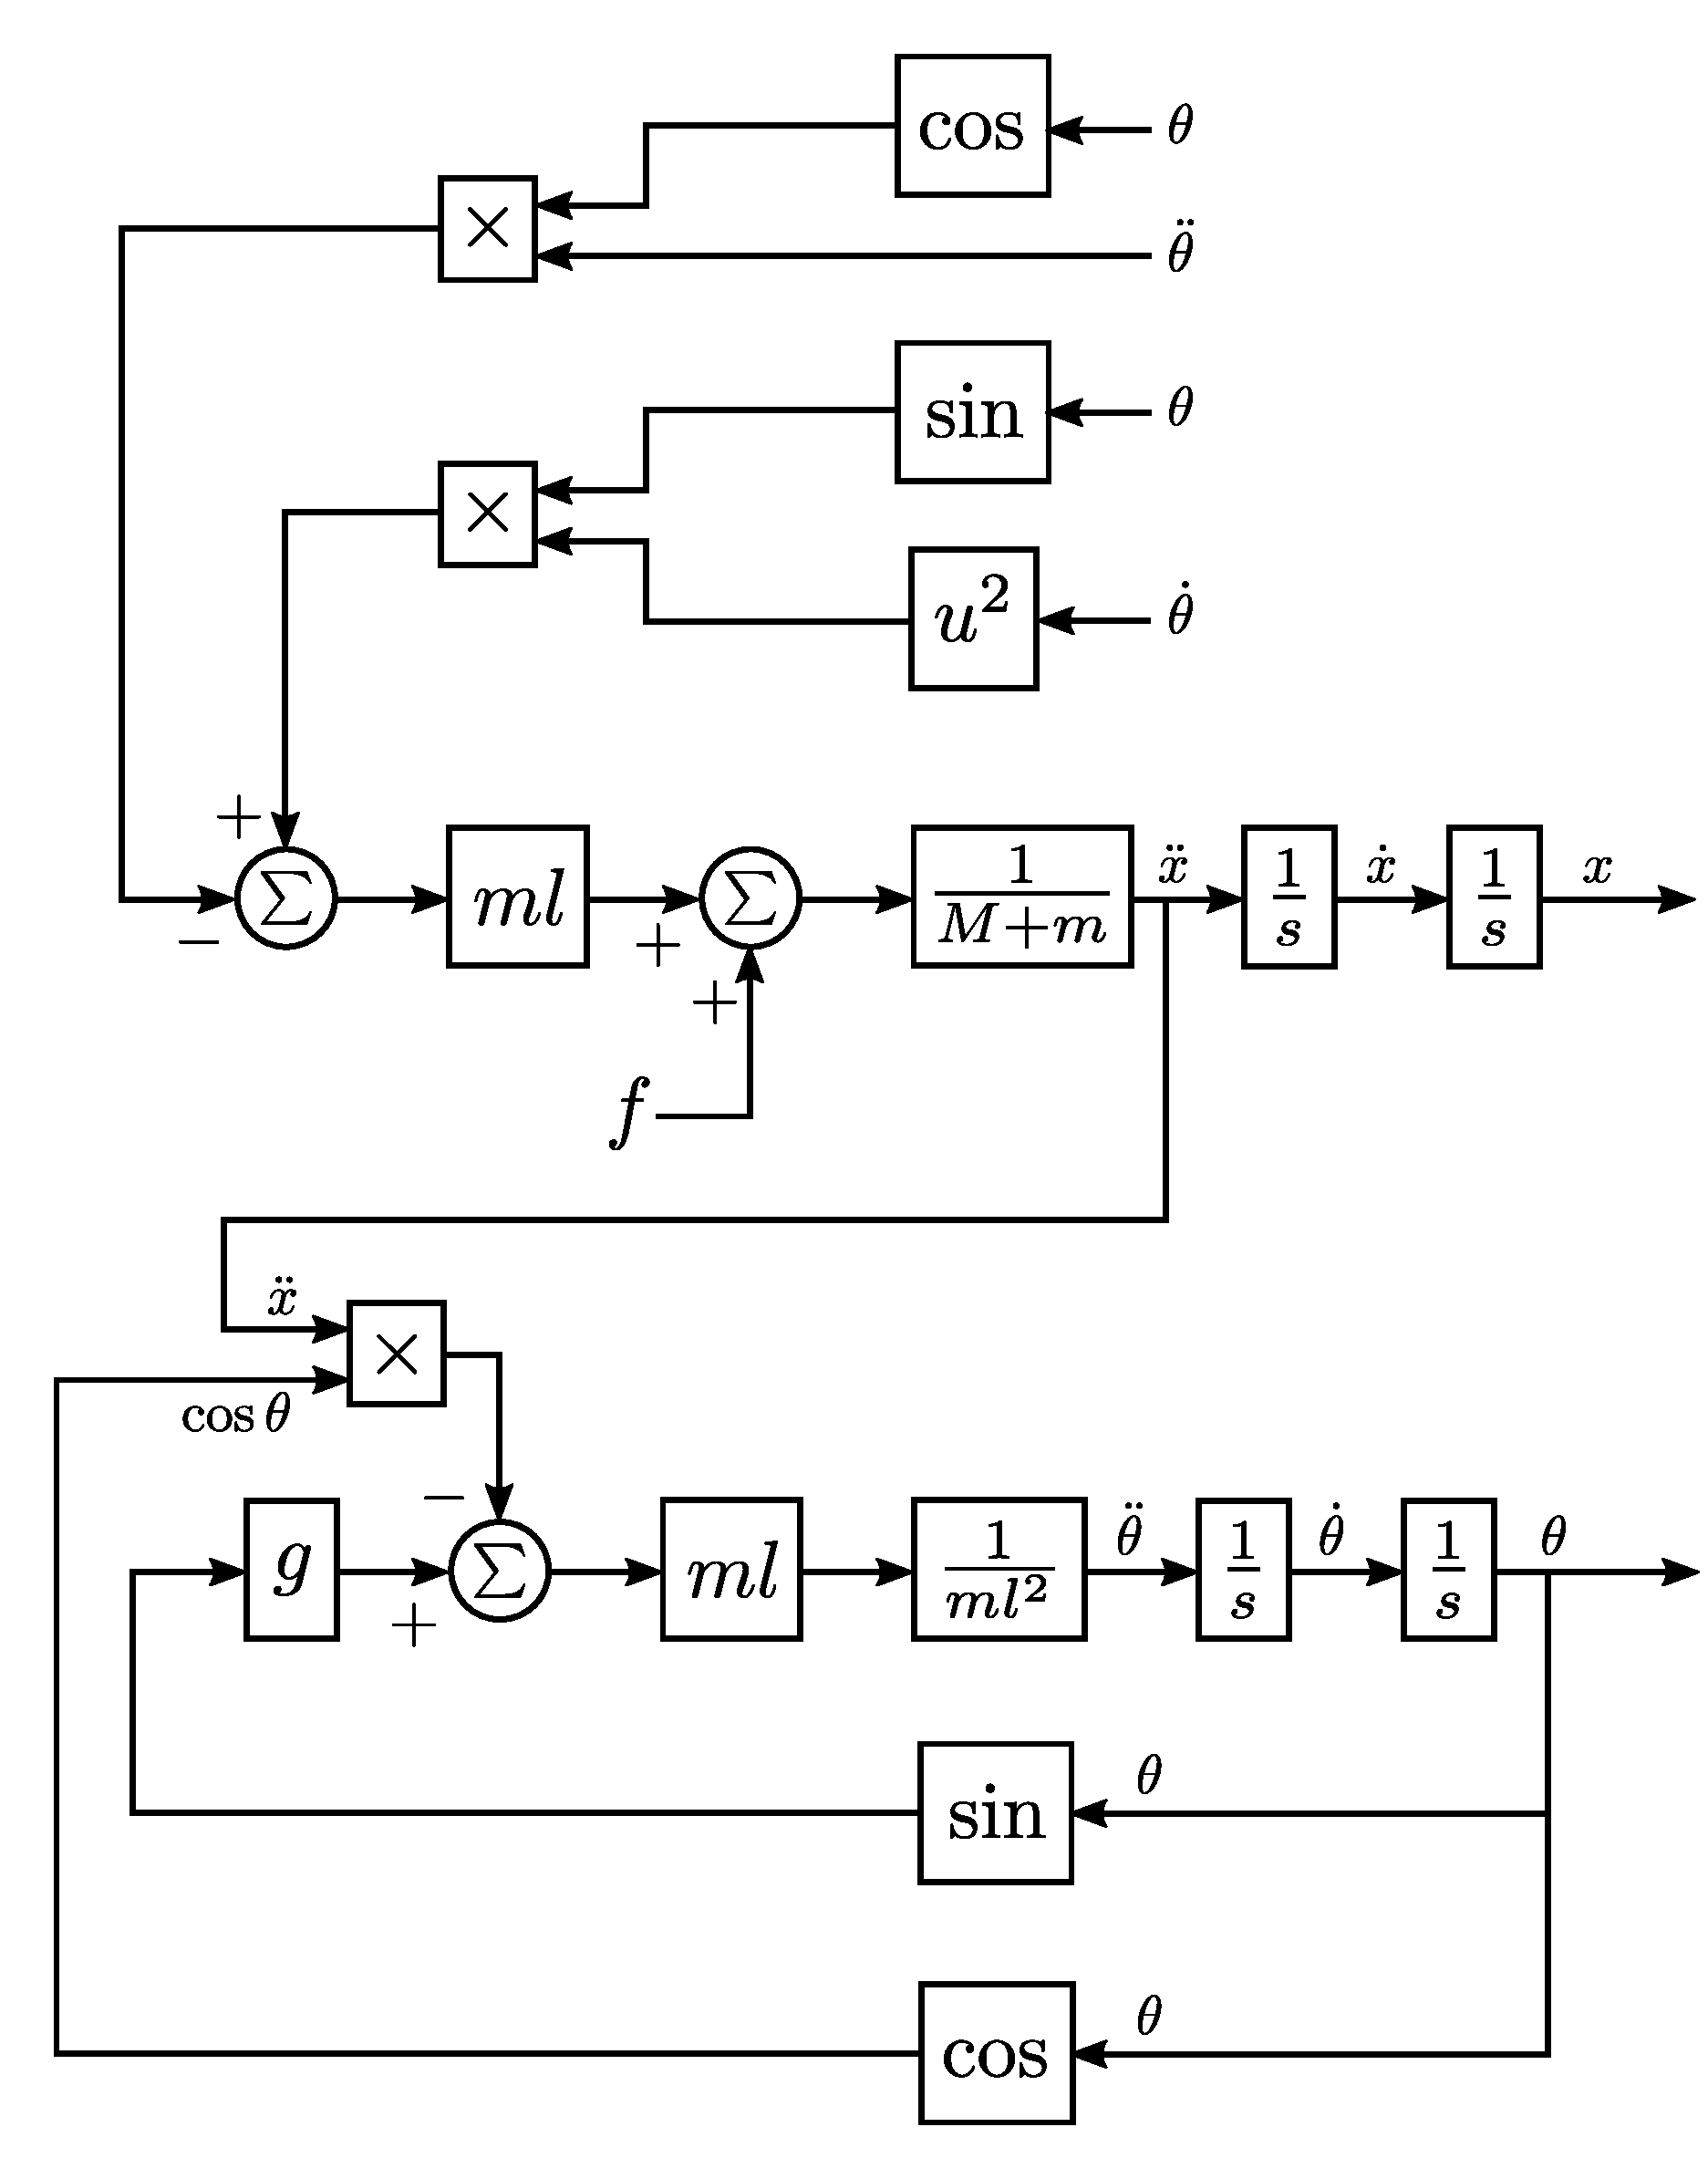
\includegraphics[width=.5\textwidth]{figures/blockDiagram}
  \caption{A block diagram derived from the dynamic equations, later used for simulation. The four signals in the top, $\theta$, $\dot{\theta}$ and $\ddot{\theta}$, are drawn without explicit connection only to keep the figure clear.}
  \label{fig:blockDiagram}
\end{figure}

This is implemented in Matlab Simulink to be able to simulate the system. A graphical layer, including the obstacles, is added to the simulation to show the system in action.
\section{Newton's Method}

Excessive coordinates - freebody diagrams in \autoref{fig:freeBodyCart} and \ref{fig:freeBodyPendulum}

\begin{figure}[H]
  \hspace{-10pt}
  \captionbox
  {
    freeBodyCart
    \label{fig:freeBodyCart}
  }
  {
    \hspace{-1cm}
    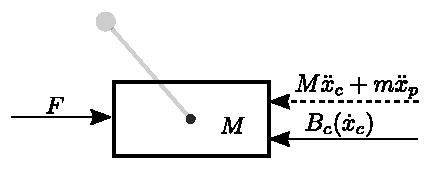
\includegraphics[width=.4\textwidth]{figures/freeBodyCart}
  }
  \hspace{20pt}
  \captionbox 
  {
    freeBodyPendulum
    \label{fig:freeBodyPendulum}
  }
  {
    \hspace{-1cm}
    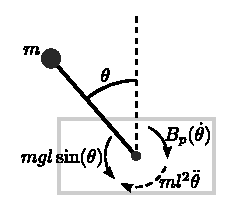
\includegraphics[width=.28\textwidth]{figures/freeBodyPendulum}
  }  
\end{figure}
%
Newton's second law for the cart along $x_c$. Freebody diagram in \autoref{fig:freeBodyCart}
\begin{flalign}
  M\ddot{x}_c + m\ddot{x}_p &= F - B_c(\dot{x}_c) &
  \label{eq:newtonAlongX}
\end{flalign}
%
Applying Newton's second law for rotational motion. Freebody diagram in \autoref{fig:freeBodyPendulum}
\begin{flalign}
  ml^2 \ddot{\theta} &= mgl \sin \theta - B_p(\dot{\theta}) &
  \label{eq:newtonRotation}
\end{flalign}
%
Relation of D'alumbert forces for the pendulum decomposed as tangential forces,
\begin{flalign}
  - m\ddot{x}_p \cos \theta - m\ddot{y}_p \sin \theta &= ml \ddot{\theta} &
  \label{eq:dalumbert}
\end{flalign}
%
To combine \autoref{eq:dalumbert} and \ref{eq:newtonRotation}, \autoref{eq:dalumbert} is written as torques,
\begin{flalign}
  - ml\ddot{x}_p \cos \theta - ml\ddot{y}_p \sin \theta &= ml^2 \ddot{\theta} &
  \label{eq:dalumbertTorques}
\end{flalign}
%
\autoref{eq:dalumbert} and \ref{eq:newtonRotation} are combined,
\begin{flalign}
  - ml\ddot{x}_p \cos \theta - ml\ddot{y}_p \sin \theta &=  mgl \sin \theta - B_p(\dot{\theta}) &
  \label{eq:dalumbertTorquesANDnewtonRotation}
\end{flalign}
%
The system dynamics is then represented using excessive coordinates by the following set of equations:
\begin{flalign}
  \begin{cases}
    - ml\ddot{x}_p \cos \theta - ml\ddot{y}_p \sin \theta =  mgl \sin \theta - B_p(\dot{\theta}) & \\
    M\ddot{x}_c + m\ddot{x}_p = F - B_c(\dot{x}_c) &
  \end{cases}  & \unit{\cdot}
  \label{eq:excessiveCoordinates}
\end{flalign}
%
Writing the excessive coordinates, \autoref{fig:excessiveCoordinates}, in therms of the generalized coordinates, \autoref{fig:mechanicalDrawing},
\begin{flalign}
  \begin{cases}
    x_c &=  x  \\
    y_c &=  0  
  \end{cases} &
    \hspace{20pt}
  \begin{cases}
    x_p =  x - l\sin \theta \\
    y_p =  l\cos \theta
  \end{cases}  &
  \label{eq:coordinateTransformation}
\end{flalign}
%
Finding the derivatives for the transformation,
\begin{flalign}
  \begin{cases}
    \dot{x}_p &= \dot{x} - l\cos \theta \dot{\theta} \\
    \dot{y}_p &= -l\sin \theta \dot{\theta}
  \end{cases} &
    \hspace{20pt}
  \begin{cases}
    \ddot{x}_p = \ddot{x} + l \sin \theta \dot{\theta}^2 - l\cos \theta \ddot{\theta} \\
    \ddot{y}_p = -l\cos \theta \dot{\theta}^2  -l\sin \theta \ddot{\theta}
  \end{cases}  &
  \label{eq:transformationDerivatives}
\end{flalign}
%
Rewriting \autoref{eq:excessiveCoordinates} in generalized coordinates using the cooredinate transformation from \autoref{eq:coordinateTransformation} and \ref{eq:transformationDerivatives} yields,
\begin{flalign}
  \begin{cases}
     - ml( \ddot{x} + l \sin \theta \dot{\theta}^2 -l\cos \theta \ddot{\theta} ) \cos \theta - ml ( -l \cos \theta \dot{\theta}^2 -l\sin \theta \ddot{\theta} ) \sin \theta =  mgl \sin \theta - B_p(\dot{\theta}) & \\
     M\ddot{x} + m( \ddot{x} + l\sin \theta \dot{\theta}^2 - l \cos \theta \ddot{\theta} ) = F - B_c(\dot{x}) &
  \end{cases} && \nonumber
\end{flalign}
\vspace{-14pt}
\begin{flalign}
  \begin{cases}
   ml^2 \ddot{\theta} - ml\cos \theta \ddot{x} - mgl \sin \theta &= - B_p(\dot{\theta}) \\
  ( M + m ) \ddot{x} + ml\sin \theta \dot{\theta}^2 - ml\cos \theta \ddot{\theta} &= F - B_c(\dot{x})  \ \ \ \ ,
\end{cases} & \unit{\cdot}
\label{eq:generalizedCoordinates}
\end{flalign}
%
which is the final dynamic equations for the cart pendulum system.
\subsection{Energy Method}
The energy method is applied to find the dynamic equations starting by using excessive coordinates. The potential and kinetic energy for the pendulum is,
\begin{flalign}
  U_p &= mgh                                                           & \unit{\cdot} \\
  T_p &= \tfrac{1}{2} m \dot{x}_p^2 + \tfrac{1}{2} m \dot{y}_p^2 \ \ \ , & \unit{\cdot}
  \label{eq:pendulumEnergy}
\end{flalign}
\begin{where}\\
  \va{ U_p   }{is the potential energy of the pendulum}    {\cdot}
  \va{ T_p   }{is the kinetic energy of the pendulum}      {\cdot}
  \va{ h     }{is the height of the pendulum point mass}   {m}
\end{where}

where the height, $h$, is given in relation to the pendulum at rest at $\theta = \pm \pi n$ by,
\begin{flalign}
  h &= l( 1 + \cos \theta ) \ \ \ . & \unit{\cdot}
  \label{eq:height}
\end{flalign}

The potential and kinetic energy in excessive coordinates for the cart is,
\begin{flalign}
  U_c &= 0           & \unit{\cdot} \\
  T_c &= \tfrac{1}{2} M \dot{x}_c^2   \ \ \ . & \unit{\cdot}
  \label{eq:cartEnergy}
\end{flalign}
\begin{where}
  \va{ U_c               }{is the potential energy of the cart}                    {\cdot}
  \va{ T_c               }{is the kinetic energy of the cart}                      {\cdot}
\end{where}

There is no potential energy for the cart as it is constrained at $y_c=0$.\\
The combined energies for the system in excessive coordinates is then,
\begin{flalign}
  U &= mgl( 1 + \cos \theta ) + 0    & \unit{\cdot} \\
  T &= \tfrac{1}{2} m \dot{x}_p^2 + \tfrac{1}{2} m \dot{y}_p^2  + \tfrac{1}{2} M \dot{x}_c^2 \ \ \ , & \unit{\cdot}
  \label{eq:excessivePotentialAndKinetic}
\end{flalign}
%
Using the coordinate transformation from \autoref{eq:coordinateTransformation} and \ref{eq:transformationDerivatives} to obtain the energies of the system in generalized coordinates,
\begin{flalign}
  \begin{cases}
    U &= mgl( 1 + \cos \theta ) + 0 \\
    T &= \frac{1}{2} m ( \dot{x} - l\cos \theta \dot{\theta} )^2 + \frac{1}{2} m ( -l\sin \theta \dot{\theta} )^2  + \frac{1}{2} M \dot{x}^2 
  \end{cases} && \nonumber
\end{flalign}
\vspace{-14pt}
\begin{flalign}
  \begin{cases}
    U &= mgl( 1 + \cos \theta )     \\
    T &= \frac{1}{2} ( M + m ) \dot{x}^2 - m \dot{x} l \cos \theta \dot{\theta} + \frac{1}{2} m l^2 \dot{\theta}^2 \ \ \ , 
  \end{cases} & \unit{\cdot}
  \label{eq:generalizedPotentialAndKinetic}
\end{flalign}

By \autoref{eq:generalizedPotentialAndKinetic} the Lagrangian becomes,
%
\begin{flalign}
  \cal{L} &= T - U && \nonumber \\ 
  \cal{L} &= \tfrac{1}{2} ( M + m ) \dot{x}^2 - m \dot{x} l \cos \theta \dot{\theta} + \tfrac{1}{2} m l^2 \dot{\theta}^2 - m g l( 1 + \cos \theta ) \ \ \ . & \unit{N \cdot m}
  \label{eq:lagrangian}
\end{flalign}
%
\begin{where}
  \va{ \cal{L}           }{is the Lagrangian}                          {N \cdot m}
\end{where}

From the energy method\fxnote{source and thermonology on energy method} we find the dynamic equations by,
%
\begin{flalign}
  \frac{\partial \cal{L}}{\partial \vec{q}} - \frac{d}{dt}  \frac{\partial \cal{L}}{\partial \vec{\dot{q}}}  &=  0 \ \ \ . &&
  \label{eq:energyMethod}
\end{flalign}
%
\begin{where}
  \va{ \vec{q}         }{is the generalized coordinates, $[\ \theta\ \ x\ ]^{T}$}             {}
  \va{ \vec{\dot{q}}   }{is the generalized velocities, $[\ \dot{\theta}\ \ \dot{x}\ ]^{T}$} {}
\end{where}

In order to include external forces \fxnote{add formal mumbojumbo} d'Alambert principle,
\begin{flalign}
  \frac{d}{dt}  \frac{\partial \cal{L}}{\partial \vec{\dot{q}}} - \frac{\partial \cal{L}}{\partial \vec{q}}  &=  \vec{Q} \ \ \ . &&
  \label{eq:energyMethodWith external forces}
\end{flalign}
%
\begin{where}
  \va{ \vec{Q}   }{is the external forces, $[\ -B_p(\dot{\theta})\ \ F - B_c(\dot{x})\ ]^{T}$}   {}
\end{where}



For yields the final two dynamic equations, one for each of the generalized coordinates,
%
\begin{flalign}
  \begin{cases}
     \frac{d}{dt}  \frac{\partial \cal{L}}{\partial \dot{\theta}} - \frac{\partial \cal{L}}{\partial \theta}  &= m \dot{x} l \sin \theta \dot{\theta} - m l \cos \theta \ddot{x} + m l^2 \ddot{\theta} - m \dot{x} l \sin \theta \dot{\theta} - m g l \sin \theta   \\ %\unit{N \cdot m}  \\
     \frac{d}{dt}  \frac{\partial \cal{L}}{\partial \dot{x}}  - \frac{\partial \cal{L}}{\partial x} &=  ( M + m )\ddot{x} + m l \sin \theta \dot{\theta}^2 - m l \cos \theta \ddot{\theta} - 0 \\ %\unit{N \cdot m}
  \end{cases} \nonumber &&
\end{flalign}
\vspace{-14pt}
\begin{flalign}
  \begin{cases}
    m l^2 \ddot{\theta} - m l \cos \theta \ddot{x} - m g l \sin \theta  = -B_p(\dot{\theta}) & \\                      %\unit{N \cdot m}  \\
    ( M + m )\ddot{x} + m l \sin \theta \dot{\theta}^2 - m l \cos \theta \ddot{\theta}  =  F - B_c(\dot{x})  \ \ \ , &   %\unit{N \cdot m}
  \end{cases} & \unit{\cdot}
  \label{eq:energyDerivedDynamicEquations}
\end{flalign}
%
which is the same result as achieved by Newton's method, as seen by comparing \autoref{eq:generalizedCoordinates} and \ref{eq:energyDerivedDynamicEquations}.





\section{Friction and Motor Model}\label{sec:frictionModel}
In the previous, the friction is represented as functions of velocities, $B_c(\dot{x})$ and $B_p(\dot{\theta})$. The frictions are assumed to consist solely of Coulomb and viscous friction. This is a fairly simplified friction model and while it might be advantageous to include further friction dynamics, such as stiction and Stribeck friction, it is considered to be out of scope in this project.
\fxnote{friction sorurce}
%
\begin{figure}[H]
  \hspace{-10pt}
  \captionbox
  {
    coulombViscous1
    \label{fig:coulombViscous1}
  }
  {
    %\hspace{-1cm}
    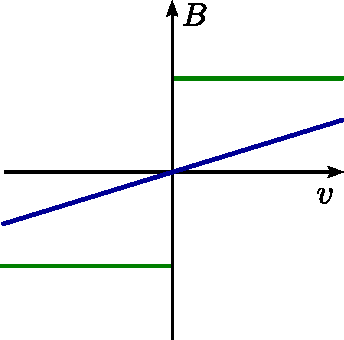
\includegraphics[width=.25\textwidth]{figures/coulombViscous1}%\vspace{-11pt}
  }
  \hspace{20pt}
  \captionbox 
  {
    coulombViscous2
    \label{fig:coulombViscous2}
  }
  {
    %\hspace{-1cm}
    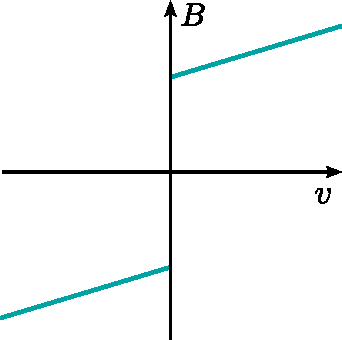
\includegraphics[width=.25\textwidth]{figures/coulombViscous2}\vspace{6pt}
  }  
\end{figure}
%
The Coulomb and viscous friction as sketched in \autoref{fig:coulombViscous1} and \ref{fig:coulombViscous2} are described by the following relations for the pendulum and cart respectively,
\begin{flalign}
  B_p(\dot{\theta}) &= b_{p,v} \dot{\theta} + \text{sgn}(\dot{\theta}) b_{p,c}        & \unit{N}  \\
  B_c(\dot{x})      &= b_{c,v} \dot{x}      + \text{sgn}(\dot{x}) b_{c,c}   \ \ \ .   & \unit{N}
  \label{eq:friction}
\end{flalign}
\begin{where}                                                                     % written out SI
  \va{ b_{p,v}   }{is the pendulum viscous friction}  {N \cdot m \cdot s}         % [kg m s^-2]
  \va{ b_{p,c}   }{is the pendulum coulomb friction}  {N \cdot m}                 % [kg s^-1]
  \va{ b_{c,v}   }{is the cart viscous friction}      {N \cdot m^{-1} \cdot s}    % [kg m^2 s^-2]
  \va{ b_{c,c}   }{is the cart coulomb friction}      {N}                         % [kg m^2 s^-1]
\end{where}

The sign-function used in \autoref{eq:friction} is undesired, as it introduces a discontinuity at zero velocity. A commonly used continuous approximation of the Coulomb friction is achieved using a tanh-function with a constant, $\text{k}_\text{tanh}$, to adjust the curve's steepness around zero.
%
\begin{figure}[H]
  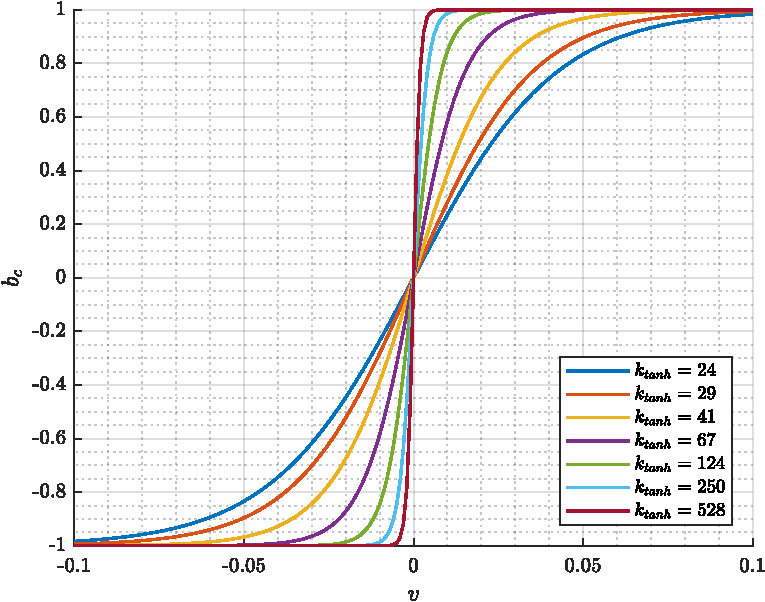
\includegraphics[width=.5\textwidth]{figures/tanhApprox}
  \caption{tanhApprox}
  \label{fig:tanhApprox}
\end{figure}

\autoref{fig:tanhApprox} shows the tanh approximation with different values of $\text{k}_\text{tanh}$. The friction parameters were estimated by a previous group who chose $\text{k}_\text{tanh} = 250$, so it makes sense to choose the same. Further, by comparing the curves in \autoref{fig:tanhApprox} the choice of $\text{k}_\text{tanh}$ seems a reasonable compromise between size of constant and steepness of the curve. The final friction model is then given by,
%
\begin{flalign}
  B_p(\dot{\theta}) &= b_{p,v} \dot{\theta} + \tanh(\text{k}_\text{tanh}\dot{\theta}) b_{p,c}        & \unit{N}  \\
  B_c(\dot{x})      &= b_{c,v} \dot{x}      + \tanh(\text{k}_\text{tanh}\dot{x}) b_{c,c}   \ \ \ .   & \unit{N}
  \label{eq:frictionTanh}
\end{flalign}

The input force so far is represented by $F$, which is directly applied in the positive $x$ direction on the cart. As seen in the beginning of this chapter in \autoref{fig:systemSetup}, this force is applied by a motor mounted with a belt on pulleys.
Because the motor control unit\fxnote{refer system description} is set up in current control mode the electrical motor dynamics are already accounted for. The controllable input is therefore the motor current, $i_a$. The torque, $\tau_m$ of the motor is modeled as directly proportional to the motor current by a torque constant, $k_\tau$, as stated in \textit{Motors} \autoref{sec:motors},
%
\begin{flalign}
  \tau_m &= k_\tau i_a       & \unit{N \cdot m}  
  \label{eq:motorTorque}
\end{flalign}

To translate this torque to the belt it is divided by the radius, $r$, of the pulley,
\begin{flalign}
  F &= \tfrac{1}{r} k_\tau i_a       & \unit{N}  
  \label{eq:motorForce}
\end{flalign}



\section{Parameters}
As mentioned, some parameters could not be measured directly. These parameter were estimated by a previous group\fxnote{reference to their thesis}. A table of the values they estimated along with directly measurable values are stated in \autoref{table:systemParameters}.

\begin{table}[H]
  \begin{tabular}{|lp{.4cm}|l|l|l|}
    \hline %--------------------------------------------------------------------------------
    \textbf{Parameter}        &   & \textbf{Notation} & \textbf{Quantity} & \textbf{Unit} \\
    \hline %--------------------------------------------------------------------------------
    Pendulum Mass             &   &   $m$             &                   &  kg           \\
    \hline %--------------------------------------------------------------------------------
    Cart Mass                 & * &   $M$             &                   &  kg           \\
    \hline %--------------------------------------------------------------------------------
    Rod Length                &   &   $l$             &                   &  m            \\
    \hline %--------------------------------------------------------------------------------
    Pulley Radius             &   &   $r$             &                   &  m            \\
    \hline %--------------------------------------------------------------------------------
    Cart Coulomb Friction     & * &   $b_{c,c}$       &                   &  N            \\
    \hline %--------------------------------------------------------------------------------
    Cart Viscous Friction     & * &   $b_{c,v}$       &                   &  N$\cdot$m$^{-1}\cdot$s \\
    \hline %--------------------------------------------------------------------------------
    Pendulum Coulomb Friction & * &   $b_{p,c}$       &                   &  N$\cdot$m              \\
    \hline %--------------------------------------------------------------------------------
    Pendulum Viscous Friction & * &   $b_{p,v}$       &                   &  N$\cdot$m$\cdot$s      \\
    \hline %--------------------------------------------------------------------------------
  \end{tabular}
  \caption{'*' indicates that the parameter is estimated.\label{table:systemParameters}}
\end{table}

Though the inertia of the rotor is stated in the datasheet of the motor, see \textit{Hardware} \autoref{sec:hardware}, the added inertia and mass of from the pulley and belt is unknown. Further, both viscous and Coulomb friction on the cart are assumed purely translational. Similarly, though the weights of motor and motor controller mounted on the cart are known, the collective weight of the cart is unknown. For these reasons, the cart weight, viscous and Coulomb friction were estimated by the previous group such that they include friction and inertia added by the motor, belt and pulleys.\fxnote{reference to old report}

%\section{Simulation and Verification}

A block diagram is derived in \autoref{fig:blockDiagram} from %\autoref{eq:dynamicEquation1} and \autoref{eq:dynamicEquation2}.

\begin{figure}[H]
  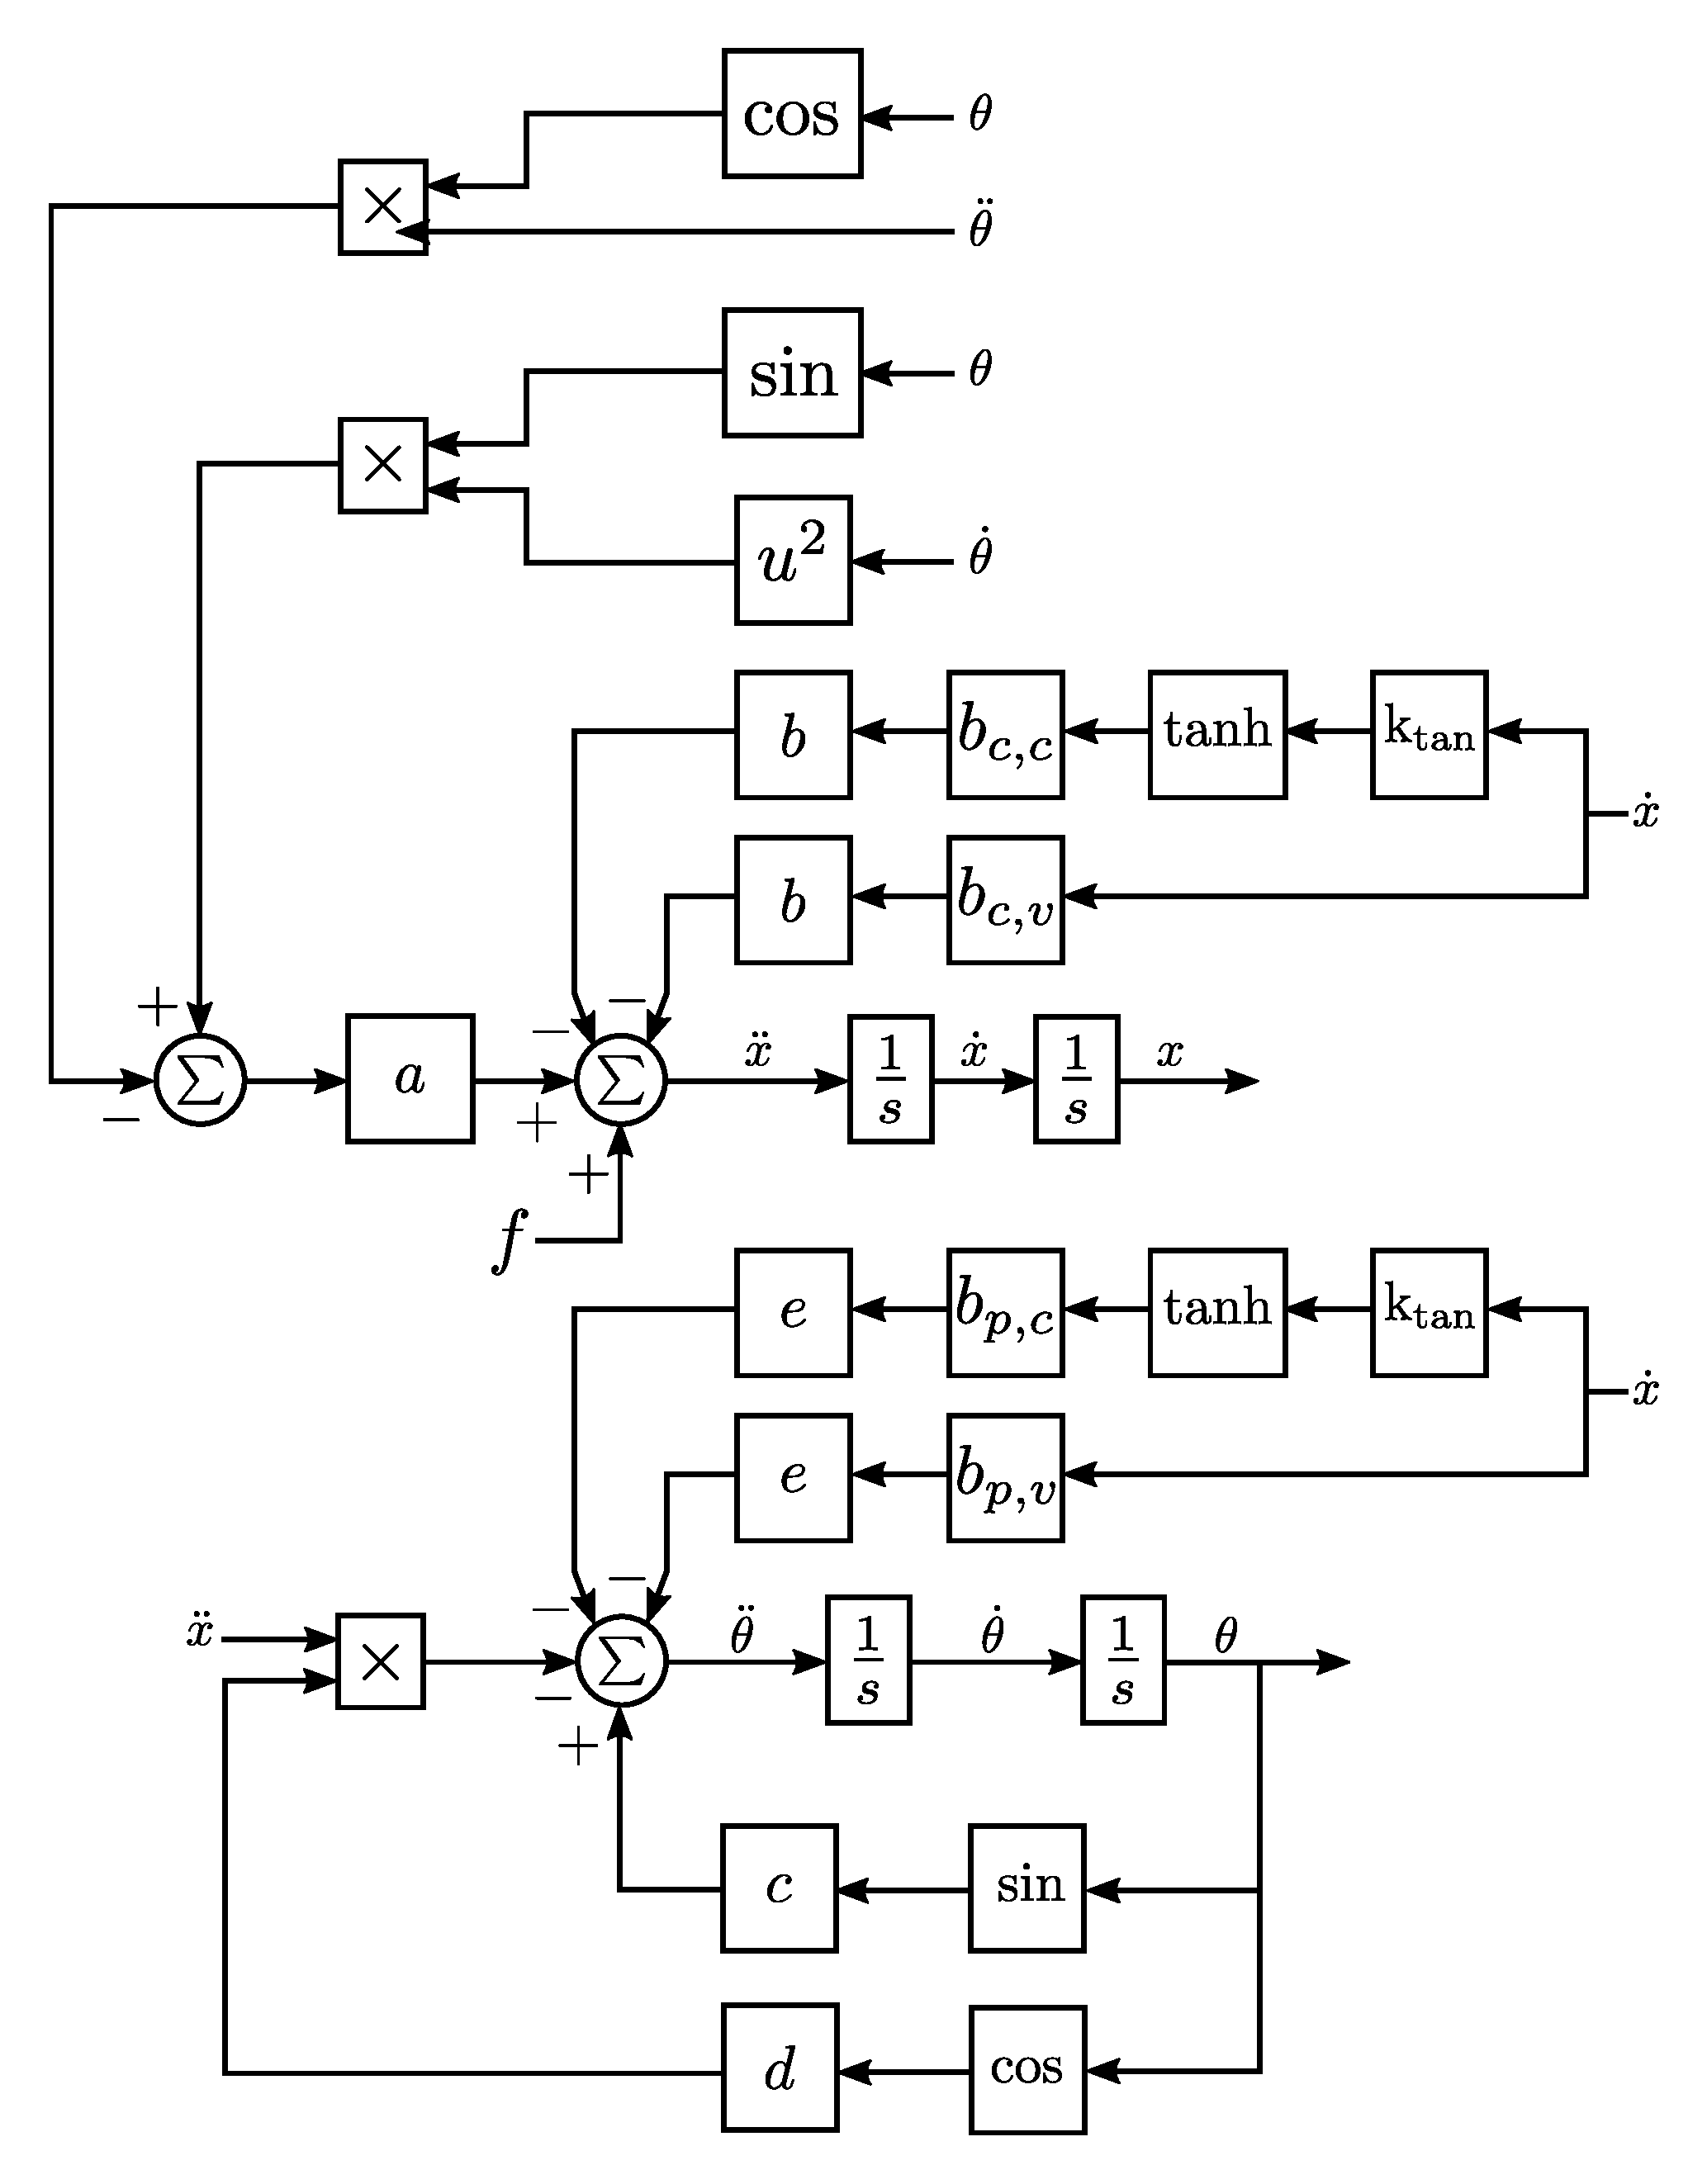
\includegraphics[width=.7\textwidth]{figures/blockDiagramWithFriction}
  \caption{A block diagram derived from the dynamic equations, later used for simulation. Five signal connections, from $\dot{\theta}$, $\ddot{\theta}$, $\ddot{x}$ and two from $\theta$, are drawn without explicit connection to keep the figure clear.}
  \label{fig:blockDiagram}
\end{figure}

This is implemented in Matlab Simulink to simulate the system. A graphical layer, including the obstacles, is added to the simulation to show the system in action.
%\section{Nonlinear Analysis}
In this section the nonlinear nature of the system is studied.\fxnote{name the tools used in the section}

It is possible to map trajectories in the ($\theta$, $\dot{\theta}$)-plane assuming no applied force. To construct the phase portrait the dynamic equations, \autoref{eq:dynamicEquation1} and \autoref{eq:dynamicEquation1}, are combined. First $\ddot{x}$ is isolated in \autoref{eq:dynamicEquation2},
%
\begin{flalign}
  \ddot{x} &= - \frac{m l \cos \theta \ddot{\theta}}{M + m}  + \frac{m l \sin \theta \dot{\theta}^2}{M + m} + \frac{f}{M + m}   \ \ \ . & %\unit{N \cdot m}
  \label{eq:dynamicEquationX}
\end{flalign}

This expression for $\ddot{x}$ is then substituted in \autoref{eq:dynamicEquation1} to obtain the dynamics in therms of the angle and its derivatives.
%
\begin{flalign}
  m l \cos \theta
  \left(
    - \frac{m l \cos \theta \ddot{\theta}}{M + m}  + \frac{m l \sin \theta \dot{\theta}^2}{M + m} + \frac{f}{M + m}
  \right)
  + m l^2 \ddot{\theta} - m l g \sin \theta &=  0   \ \ \ . & %\unit{N \cdot m}
  \label{eq:dynamicEquationSubsX}
\end{flalign}

Rearranging yields,
%
\begin{flalign}
  \left( m l^2 - \frac{m^2 l^2}{M + m} \cos ^2 \theta \right) \ddot{\theta}
  + \left( \frac{m^2 l^2}{M + m} \sin \theta \cos \theta \right) \dot{\theta}^2
  + f \frac{m l}{M + m} \cos \theta - m g l \sin \theta &=  0   \ \ \ , & %\unit{N \cdot m}
  \label{eq:alphaBetaGamma}
\end{flalign}
%
which is the reduced system on the general form,
%
\begin{flalign}
  \alpha (\theta) \ddot{\theta} + \beta (\theta) \dot{\theta}^2 + \gamma (\theta) &=  0   \ \ \ , & %\unit{N \cdot m}
  \label{eq:alphaBetaGammaGeneral}
\end{flalign}
%
where, $\alpha (\theta)$, $\beta (\theta)$ and $\gamma (\theta)$ are the scalar functions of $\theta$ from \autoref{eq:alphaBetaGamma}.

Finally the reduced system on state space form, where $x_1 = \theta$ and $x_2 = \dot{\theta}$,
%
\begin{flalign}
  \dot{x_1}  &=  x_2  \nonumber \\
  \dot{x_2}  &=  -\frac{\beta (x_1)}{\alpha (x_1)} x_2^2 -\frac{\gamma (x_1)}{\alpha (x_1)}   \ \ \ . & %\unit{N \cdot m}
  \label{eq:stateSpaceThetaDynamics}
\end{flalign}

In \autoref{fig:phasePortrait} the phase portrait is generated using pplane8.\fxnote{source of pplane8.m}

\begin{figure}[H]
  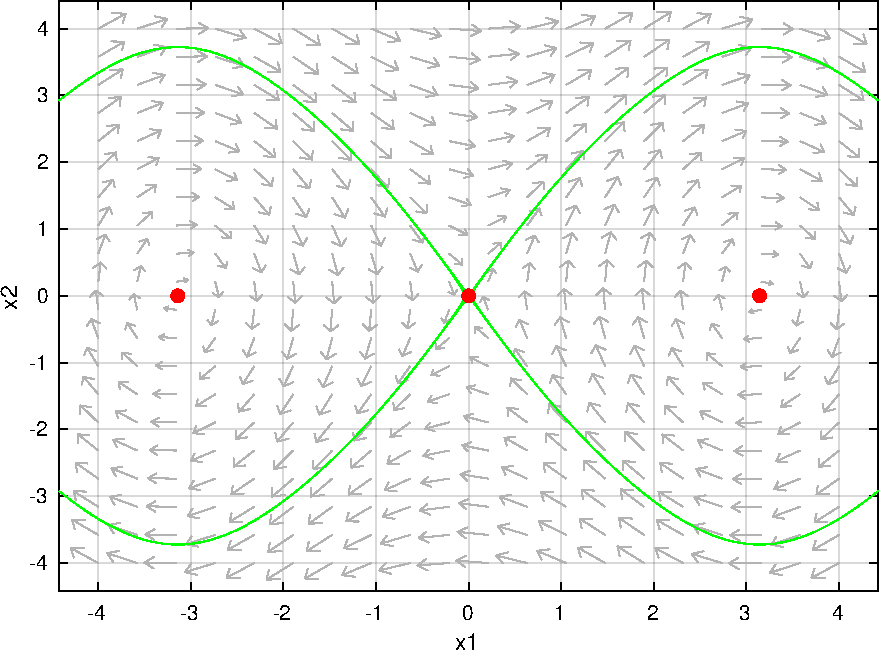
\includegraphics[width=.8\textwidth]{figures/systemPhasePortrait}
  \caption{Phase portrait of the $\theta$-dynamics, where $x_1 = \theta$ and $x_2 = \dot{\theta}$. The equilibrium points are shown in red and the unstable orbits at the saddle point are indicated in green.}
  \label{fig:phasePortrait}
\end{figure}

As there is no friction in the system the pendulum will maintain one particular orbit around one of the center equilibrium points so long as the initial value is within the confines of the unstable orbit at the saddle point. This means that the pendulum will oscillate without loss of amplitude if the initial angular velocity, $\dot{\theta}$, is zero or at least places the starting point within the saddle.\\
If on the other hand the initial value of $\dot{\theta}$ is positive and $\theta$ is zero (upright position), then the pendulum will do full rotations around the cart, thus continuously increasing the angle.

If a force is imposed on the system it can change the phase portrait, allowing for other possible trajectories. This is further investigated in the following chapter.


%---------- Chapter 5 ---------------------------------------- Nonlinear Control
\chapter{Nonlinear Control}
The control objective is to stabilize the pendulum at $\theta = 0$. To achieve this objective a sliding mode controller is designed for the cart pendulum system. To do so the system is transformed into a \textit{regular form} presented in this chapter along with the sliding mode design.
\section{System Transformation}
To transform the system into a \textit{regular form} which can be used for design of the sliding mode controller, the system is first presented on nonlinear state space form, from \autoref{eq:energyDerivedDynamicEquations},
%
\begin{flalign}
  \begin{bmatrix}
    m l^2              & -m l \cos \theta  \\
    -m l \cos \theta   & M + m
  \end{bmatrix}
  \begin{bmatrix}
    \ddot{\theta}  \\
    \ddot{x}
  \end{bmatrix}
  +
  \begin{bmatrix}
    -m g l \sin \theta  \\
    m l \sin \theta \dot{\theta}^2
  \end{bmatrix}
  &=
  \begin{bmatrix}
    -B_p(\dot{\theta})  \\
     F - B_c(\dot{x})
  \end{bmatrix} &
  \label{eq:nonlinearSS1}
\end{flalign}
%
By rearranging \autoref{eq:nonlinearSS1}, 
\begin{flalign}
  \begin{bmatrix}
    m l^2              & -m l \cos \theta  \\
    -m l \cos \theta   & M + m
  \end{bmatrix}
  \begin{bmatrix}
    \ddot{\theta}  \\
    \ddot{x}
  \end{bmatrix}
  +
  \begin{bmatrix}
    0  \\
    m l \sin \theta \dot{\theta}^2
  \end{bmatrix}
  +
  \begin{bmatrix}
    B_p(\dot{\theta})  \\
    B_c(\dot{x})
  \end{bmatrix}
  +
  \begin{bmatrix}
  -m g l \sin \theta  \\
  0
  \end{bmatrix}
  &=
  \begin{bmatrix}
    0  \\
    F
  \end{bmatrix} \ \ \ , &
\end{flalign}
%
the achieved form is that of the general dynamic equations for an m-link robot, \cite{MWSpong, LSciavicco}
\begin{flalign}
  \vec{M}(\vec{q})\vec{\ddot{q}} + \vec{C}(\vec{q},\vec{\dot{q}}) + \vec{B}(\vec{\dot{q}}) + \vec{G}(\vec{q}) &= \vec{F} \ \ \ . &
\end{flalign}
\begin{where}
  \va{ \vec{M}(\vec{q})\vec{\ddot{q}}  }{is the inertia matrix}                    {}
  \va{ \vec{C}(\vec{q},\vec{\dot{q}})  }{is the Coriolis and centrifugal effects}  {}
  \va{ \vec{B}(\vec{\dot{q}})          }{is the friction}                          {}
  \va{  \vec{G}(\vec{q})               }{is the force due to gravity}              {}
  \va{  \vec{F}                        }{is the input force}                       {}
\end{where}

Isolating the accelerations,
\begin{flalign}
  \vec{\ddot{q}}
  &=
  \vec{M}^{-1}(\vec{q})
  \left(
    \vec{F} -\vec{C}(\vec{q},\vec{\dot{q}}) -\vec{B}(\vec{\dot{q}}) -\vec{G}(\vec{q})
  \right) \ \ \ , &
\end{flalign}
%
and choosing the state vector to be $ [\ x_1\ x_2\ x_3\ x_4\ ]^T = [\ \theta\ x\ \dot{\theta}\ \dot{x}\ ]^T $, the nonlinear state space representation is then,
%
\begin{flalign}
  \begin{bmatrix}
    \dot{x_1} \\
    \dot{x_2} \\
    \dot{x_3} \\
    \dot{x_4}
  \end{bmatrix}
&=
  \begin{bmatrix}
    x_3  \\
    x_4  \\
    \vec{M}^{-1}(x_1)
    \left(
    -\vec{C}(x_1,x_3) -\vec{B}(x_3,x_4) -\vec{G}(x_1)
    \right)
  \end{bmatrix}
  +
  \begin{bmatrix}
    0  \\
    0  \\
    \vec{M}^{-1}(x_1)   \begin{bmatrix}
                          0  \\
                          F
                        \end{bmatrix}
  \end{bmatrix} \ \ \ , &
\end{flalign}
%
where,
\begin{flalign}
  \vec{M}^{-1}
  &=
  \frac{1}{\text{det}(\vec{M})} \text{adj}(\vec{M})
  =
  \begin{bmatrix}
    \frac{(M + m)}{l^2 m ( M + m - m \cos x_1^2 )}  &  \frac{\cos x_1}{l (M + m - m \cos x_1^2)} \\
    \frac{\cos x_1}{l (M + m - m \cos x_1^2)}       &  \frac{1}{M + m - m \cos x_1^2}
  \end{bmatrix}  \ \ \ . &
\end{flalign}
%
Introducing following notation,
\begin{flalign}
  \begin{bmatrix}
    \dot{x_1} \\
    \dot{x_2} \\
    \dot{x_3} \\
    \dot{x_4}
  \end{bmatrix}
  &=
  \underbrace{ 
    \begin{bmatrix}
      x_3  \\
      x_4  \\
      f_1(\vec{x})  \\
      f_2(\vec{x})
    \end{bmatrix}
  }_{f(\vec{x})}
  +
  \underbrace{ 
    \begin{bmatrix}
      0  \\
      0  \\
      \frac{\cos x_1}{l (M + m - m \cos x_1^2)} \\
      \frac{1}{M + m - m \cos x_1^2}
    \end{bmatrix}
  }_{g(\vec{x})}
  F \ \ \ . &
  \label{eq:reducedNonlinearStateSpace}
\end{flalign}
%
where,
%
\begin{flalign}
f_1(\vec{x}) &=  \frac{(M + m) (  -B_p(x_3) + m g l \sin x_1  )}{l^2 m ( M + m - m \cos x_1^2 )}   -    \frac{\cos x_1 (  m l \sin x_1 x_3^2 + B_c(x_4)  )}{l (M + m - m \cos x_1^2)}  & \\
f_2(\vec{x}) &=  \frac{\cos x_1 (  -B_p(x_3) + m g l \sin x_1  )}{l (M + m - m \cos x_1^2)}   -   \frac{ m l \sin x_1 x_3^2 + B_c(x_4) }{M + m - m \cos x_1^2}       \ \ \ , &
\end{flalign}
%
to reduce notation in the derivation of the transformation into \textit{regular form}.

Choosing the pendulum angle as the output s.t. $y = h(\vec{x}) = x_1$, the relative degree is found by,
\begin{flalign}
\dot{y}  &= \dot{x_1} = x_3 & \\
\ddot{y} &= \dot{x_3} = f_1(\vec{x}) + \frac{\cos x_1}{l (M + m - m \cos x_1^2)} F \ \ \ , &
\end{flalign}
where the output is found in the second derivative of the output, resulting in relative degree of two, $\rho = 2$, which gives rise to the following transform \fxnote{source},
%
\begin{flalign}
T(\vec{x})
&=
\begin{bmatrix}
  \phi(\vec{x}) \\  %these are dotted lines, yea, that's LaTeX for ya, go figure..
  \begin{picture} (0,0)(0,0) \multiput(1,14)(4,0){6}{\line(2,0){2}} \end{picture}
  \psi(\vec{x})
\end{bmatrix} 
=
\begin{bmatrix}
  \phi_1(\vec{x}) \\
  \phi_2(\vec{x}) \\  %these are dotted lines, yea, that's LaTeX for ya, go figure..
  \begin{picture} (0,0)(0,0) \multiput(-5.5,14)(4,0){9}{\line(2,0){2}} \end{picture}
  h(\vec{x}) \\
  L_f h(\vec{x})
\end{bmatrix}
=
\begin{bmatrix}
  \phi_1(\vec{x}) \\
  \phi_2(\vec{x}) \\  %these are dotted lines, yea, that's LaTeX for ya, go figure..
  \begin{picture} (0,0)(0,0) \multiput(-7,14)(4,0){7}{\line(2,0){2}} \end{picture}
  x_1 \\
  x_3
\end{bmatrix}  \ \ \ , &
\end{flalign}
%
where $L_f h(\vec{x})$ is the \textit{Lie derivative} of $h(\vec{x})$ along $f(\vec{x})$. The functions $\phi_i(\vec{x})$ are chosen such that they satisfy,
\begin{flalign}
  \frac{\partial \phi_i}{\partial \vec{x} }  g(\vec{x})  &= 0 \ , \ \ \text{for} \ 1 \leq i \leq 2 \ \ \ ,& 
\end{flalign}
which ensures that the input cancels in, \fxnote{fix transition}
\begin{flalign}
 \dot{\eta} &= \frac{\partial \phi}{\partial \vec{x} } [ f(\vec{x}) + g(\vec{x}) F ] \ \ \ .& 
 \label{eq:gZeroCondition}
\end{flalign}
%
Both $\phi_1(\vec{x}) = x_1$ and $\phi_1(\vec{x}) = x_2$ would satisfy \autoref{eq:gZeroCondition}, however $\phi_1(\vec{x}) = x_1$ would result in a rank defisit in $T(\vec{x})$, so $\phi_1(\vec{x}) = x_2$ is chosen. For $\phi_2(\vec{x})$, it follows from \autoref{eq:gZeroCondition} that, 
\begin{flalign}
  \frac{\partial \phi_2}{\partial x_3 } \cdot \frac{\cos x_1}{l (M + m - m \cos x_1^2)}  &+  \frac{\partial \phi_2}{\partial x_4 } \cdot \frac{1}{M + m - m \cos x_1^2}  =  0   & \\
  \frac{\partial \phi_2}{\partial x_3 } \cdot \frac{\cos x_1}{l (M + m - m \cos x_1^2)}  &+  \frac{\partial \phi_2}{\partial x_4 } \cdot \frac{l}{l(M + m - m \cos x_1^2)}  =  0  \ \ \ . & 
  \label{eq:gZeroCondition2}
\end{flalign}
%
It is attempted to cancel the two therms in \autoref{eq:gZeroCondition2} by choosing,
\begin{flalign}
  \frac{\partial \phi_2}{\partial x_3 } &=  \frac{l}{\cos x_1} \ \ , \ \ \ \ \ \frac{\partial \phi_2}{\partial x_4 } =  -1  & 
  \label{eq:gZeroConditionCancle}
\end{flalign}
\vspace{-24pt}
\begin{flalign}
  \phi_2 &=  \frac{l}{\cos x_1} \int  d x_3  - \int  d x_4  & \\
  \phi_2 &=  \frac{l}{\cos x_1} x_3  - x_4 + \text{C}_1  \ \ \ . & 
  \label{eq:gZeroConditionIntegral}
\end{flalign}
where C$_1$ is an integration constant. It is also required that $\phi(0)=0$, so C$_1=0$, resulting in the final transformation,
%
\begin{flalign}
  T(\vec{x})
  &=
  \begin{bmatrix}
    x_2 \\
    \frac{l}{\cos x_1} x_3  - x_4 \\ 
    x_1 \\
    x_3
  \end{bmatrix}  \ \ \ . &
\end{flalign}
%
Locating the input in the derivative of the transform,
\begin{flalign}
  \frac{\partial }{\partial \vec{x} } T(\vec{x})
  &=
  \begin{bmatrix}
    \dot{x}_2 \\
    \frac{l \sin x1}{\cos ^2 x_1} \dot{x}_1 x_3 +  \frac{l}{\cos x_1} \dot{x}_3 - \dot{x}_4 \\ 
    \dot{x}_1 \\
    \dot{x}_3
  \end{bmatrix}  \ \ \ . &
\end{flalign}
The second element, $\frac{\partial }{\partial \vec{x} } T_2(\vec{x})$, is further evaluated by substitution of the state derivatives from \autoref{eq:reducedNonlinearStateSpace},
\begin{flalign}
  \frac{\partial }{\partial \vec{x} } T_2(\vec{x}) &= \frac{l \sin x1}{\cos ^2 x_1} x_3^2 +  \tfrac{l}{\cos x_1} (f_1(\vec{x}) +  \tfrac{\cos x_1}{l (M + m - m \cos x_1^2)} F)  - (f_2(\vec{x}) + \tfrac{1}{M + m - m \cos x_1^2} F) & \nonumber \\
  \frac{\partial }{\partial \vec{x} } T_2(\vec{x}) &= \frac{l \sin x1}{\cos ^2 x_1} x_3^2 +  \tfrac{l}{\cos x_1} f_1(\vec{x})  - f_2(\vec{x})  \ \ \ , &
\end{flalign}
showing that the output only appears on the fourth element in the derivative of the transformation. This leads to choosing $ [\ \eta_1\ \eta_2\ \eta_3\ \xi\ ]^T$ as the new variables, with its derivatives,
\begin{flalign}
  \begin{bmatrix}
    \dot{\eta}_1   \\
    \dot{\eta}_2   \\
    \dot{\eta}_3   \\  %these are dotted lines, yea, that's LaTeX for ya, go figure..
    \begin{picture} (0,0)(0,0) \multiput(-2,14)(4,0){3}{\line(2,0){2}} \end{picture}
    \dot{\xi}
  \end{bmatrix} 
  &=
  \overbrace{
  \underbrace{
    \begin{bmatrix}
      x_4    \\
      \frac{l \sin x1}{\cos ^2 x_1} x_3^2 +  \tfrac{l}{\cos x_1} f_1(\vec{x})  - f_2(\vec{x}) \\ 
      x_3    \\ %these are dotted lines, yea, that's LaTeX for ya, go figure..
      \begin{picture} (0,0)(0,0) \multiput(-49,14)(4,0){28}{\line(2,0){2}} \end{picture}
      f_1(\vec{x}) 
    \end{bmatrix}
  }_{f_b} }^{f_a}
  +
  \underbrace{
    \begin{bmatrix}
      0    \\
      0    \\
      0    \\  %these are dotted lines, yea, that's LaTeX for ya, go figure..
      \begin{picture} (0,0)(0,0) \multiput(4,14)(4,0){17}{\line(2,0){2}} \end{picture}
      \frac{\cos x_1}{l (M + m - m \cos x_1^2)}
    \end{bmatrix}
  }_{g_b} F  \ \ \ , &
\label{eq:regularFormWithX}
\end{flalign}
which is the \textit{regular form} where,
\begin{flalign}
  \vec{\dot{\eta}} &=  f_a(\vec{\eta},\xi)    \\
  \dot{\xi}        &=  f_b(\vec{\eta},\xi) + g_b(\vec{\eta},\xi) F    \ \ \ . &
\end{flalign}
%
The original state vector is represented using the new variables,
\begin{flalign}
  \begin{bmatrix}
    \eta_1   \\
    \eta_2   \\
    \eta_3   \\
    \xi
  \end{bmatrix} 
  &=
  \begin{bmatrix}
    x_2 \\
    \frac{l}{\cos x_1} x_3  - x_4 \\
    x_1 \\
    x_3
  \end{bmatrix} \ \ \ \ \ \ \ \ \ 
  \begin{bmatrix}
    x_1   \\
    x_2   \\
    x_3   \\
    x_4
  \end{bmatrix} 
  =
  \begin{bmatrix}
    \eta_3 \\
    \eta_1 \\ 
    \xi    \\
    \frac{l}{\cos \eta_3} \xi -\eta_2
  \end{bmatrix}  \ \ \ , &
\end{flalign}
to then formulate \autoref{eq:regularFormWithX} in therms of $ [\ \eta_1\ \eta_2\ \eta_3\ \xi\ ]^T$, \fxnote{word on diffeomorphism, inverse transform exist.. smthng.}
%
\begin{flalign}
  \begin{bmatrix}
    \dot{\eta}_1   \\
    \dot{\eta}_2   \\
    \dot{\eta}_3   \\
    \dot{\xi}
  \end{bmatrix} 
  &=
  \begin{bmatrix}
    \frac{l}{\cos \eta_3} \xi -\eta_2    \\
    \frac{l \sin \eta_3}{\cos ^2 \eta_3} \xi^2 +  \tfrac{l}{\cos \eta_3} f_1(\vec{\eta},\xi)  - f_2(\vec{\eta},\xi) \\ 
    \xi   \\
    f_1(\vec{\eta},\xi) 
  \end{bmatrix} 
  + 
  \begin{bmatrix}
    0    \\
    0    \\
    0    \\ 
    \frac{\cos \eta_3}{l (M + m - m \cos^2\eta_3)}
  \end{bmatrix} F  \ \ \ , &
\label{eq:regularFormWithEtaXi}
\end{flalign}
where,
\begin{flalign}
f_1(\vec{\eta},\xi) &=  \frac{(M + m) (  -B_p(\xi) + m g l \sin \eta_3  )}{l^2 m ( M + m - m \cos \eta_3^2 )}   -    \frac{\cos \eta_3 (  m l \sin \eta_3 \xi^2 + B_c(\frac{l}{\cos \eta_3} \xi -\eta_2)  )}{l (M + m - m \cos \eta_3^2)}  & \\
f_2(\vec{\eta},\xi) &=  \frac{\cos \eta_3 (  -B_p(\xi) + m g l \sin \eta_3  )}{l (M + m - m \cos \eta_3^2)}   -   \frac{ m l \sin \eta_3 \xi^2 + B_c(\frac{l}{\cos \eta_3} \xi -\eta_2) }{M + m - m \cos \eta_3^2}       \ \ \ , &
\end{flalign}

\fxnote{fix squared placement for sin cos}

\section{Sliding Mode}
Now, with the system on \textit{regular form}, the sliding mode controller can be designed.
The sliding manifold is chosen:
\begin{flalign}
  s &=   \xi - \phi(\vec{\eta}) = 0     \ \ \ , &
\end{flalign}
where $\phi(\vec{\eta})$ must be designed. When the system is restricted to move along $s = 0$ then $\xi = \phi(\vec{\eta})$, which means the reduced-order model,
\begin{flalign}
  \vec{\dot{\eta}} &=  f_a(\vec{\eta},\phi(\vec{\eta}))     \ \ \ , &
  \label{eq:asymStabOrigReducedOrder}
\end{flalign}
is asymptotically stable in its origin. To find a stabilizing controller, $\phi(\vec{\eta})$, for \autoref{eq:asymStabOrigReducedOrder}, the reduced-order system is linearized,
%
\begin{flalign}
  A &= \frac{\partial \vec{\dot{\eta}}}{\partial \vec{\eta}} \whereThree{\vec{\eta}=\vec{0}\ \ \ \ }{\xi=0\ \ \ \ }{\text{k}_\text{tanh}=1} \ 
  =
  \begin{bmatrix}
    0 & -1                  & 0 \\
    0 & \frac{g_{p,c}}{l m} & g \\
    0 & 0                   & 0 
  \end{bmatrix}   \ \ \ , \ \ \
  B = \frac{\partial \vec{\dot{\eta}}}{\partial \xi} \whereThree{\vec{\eta}=\vec{0}\ \ \ \ }{\xi=0\ \ \ \ }{\text{k}_\text{tanh}=1} \ 
  =
  \begin{bmatrix}
    l  \\
    \frac{-b_{p,v}-b_{p,c}}{l m}  \\
    1  
  \end{bmatrix}   \ \ \ , & 
  \label{eq:linearReducedOrder_A}
\end{flalign}
%
Using the matlab \textit{place()} command, different pole-placements were attempted, seen in \autoref{fig:reducedOrderControlMany}. The chosen pole placement is $[\ -3\ \ -5\ \ -8\ ]$ resulting in the state feedback gains, $\vec{k} = [\ -12.22\ \ 8.05\ \ 20.10\ ]$, of which the result is seen in \autoref{fig:reducedOrderControl}, where the linear simulation is achieved using \textit{lsim()} and the nonlinear using \textit{ode45}. \fxnote{fix formatting on matlab function reff.'s}
\begin{adjustwidth}{-1.2cm}{-1.2cm}
\begin{minipage}{\textwidth}
  \begin{minipage}{0.58\textwidth}
    \begin{figure}[H]
      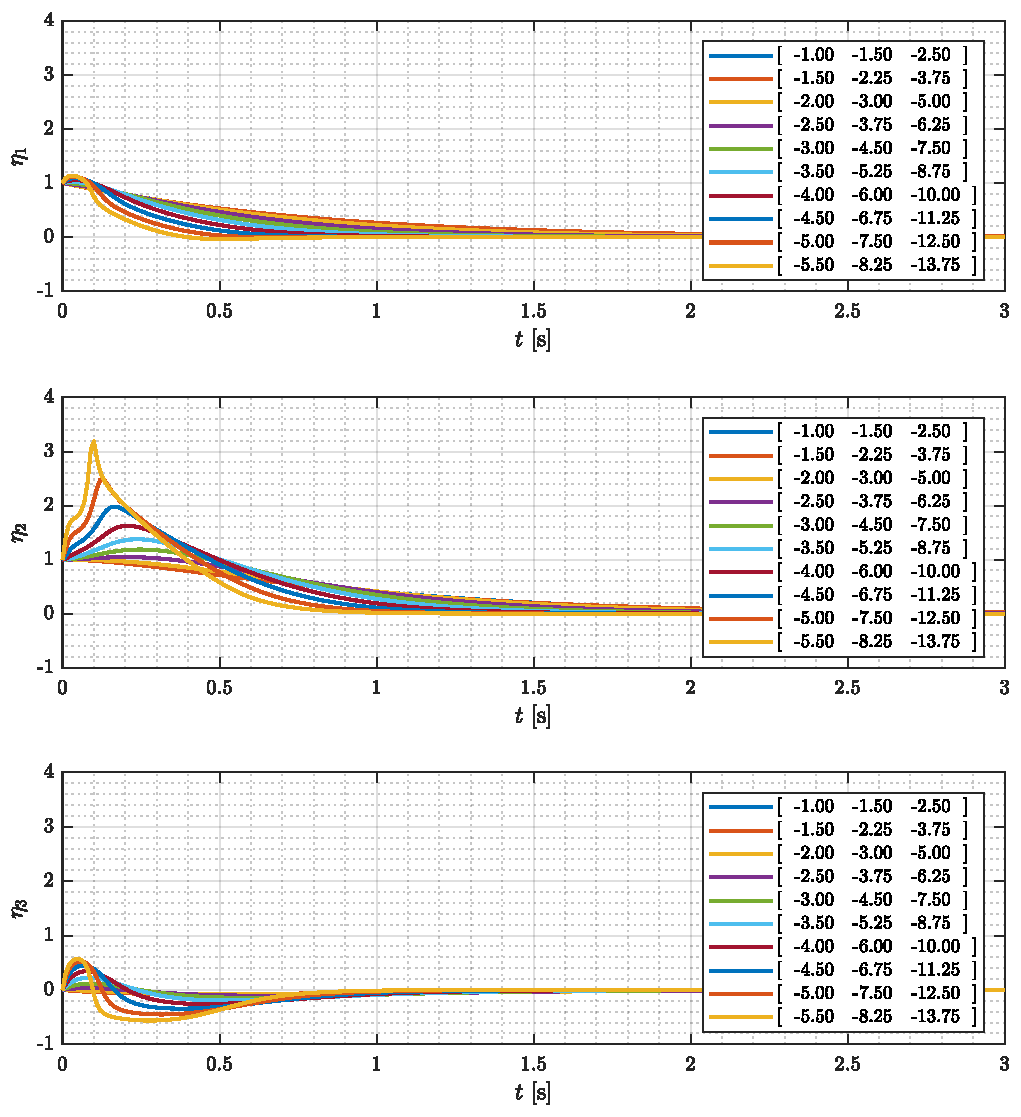
\includegraphics[width=\textwidth]{figures/reducedOrderControlMany}
      \caption{reducedOrderControlMany}
      \label{fig:reducedOrderControlMany}
    \end{figure}
  \end{minipage}
  \begin{minipage}{0.58\textwidth}
    \begin{figure}[H]
      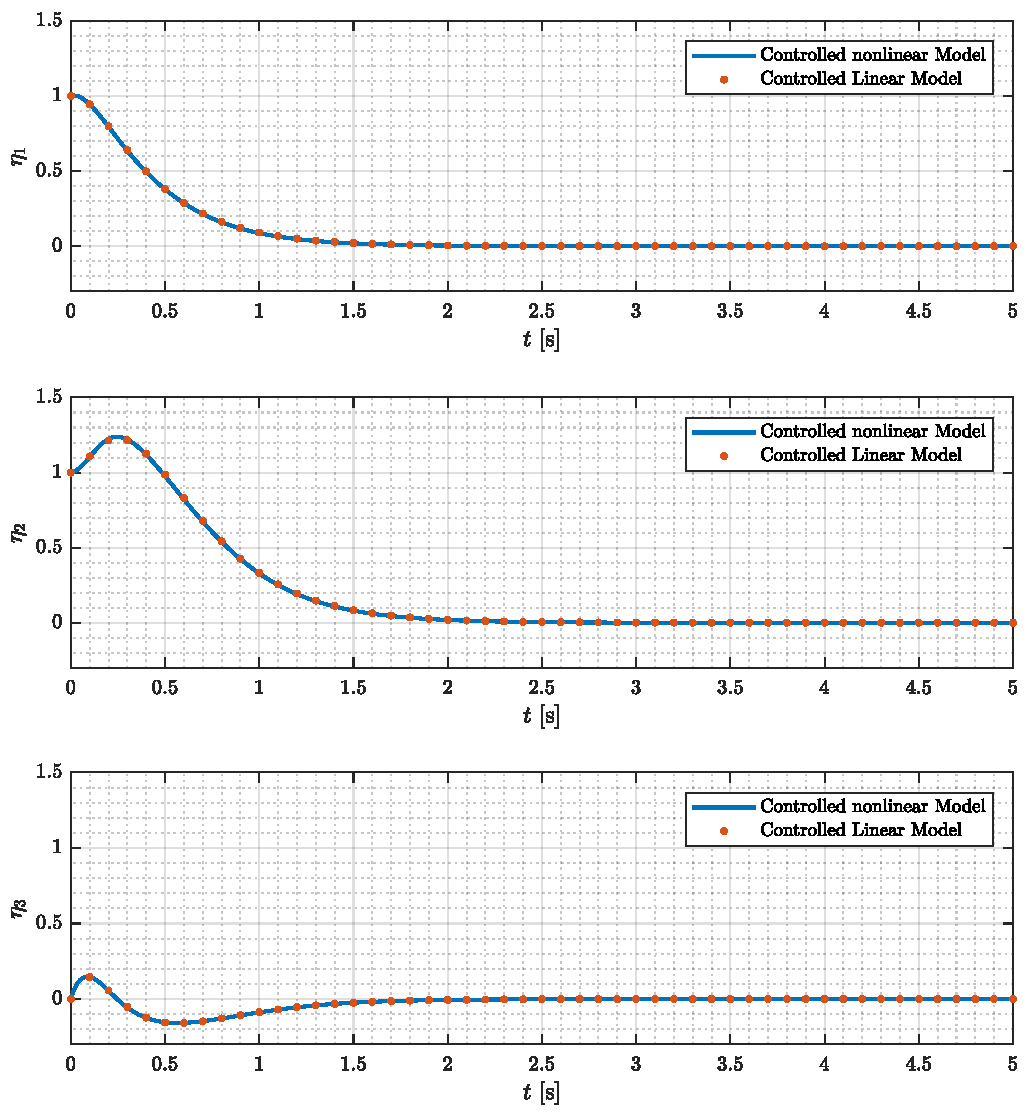
\includegraphics[width=\textwidth]{figures/reducedOrderControl}
      \caption{reducedOrderControl}
      \label{fig:reducedOrderControl}
    \end{figure}
  \end{minipage}
\end{minipage}
\end{adjustwidth}
With the reduced-order system stabilized by,
\begin{flalign}
  \phi(\vec{\eta}) &=   - \vec{k} \vec{\eta}  \ \ \ , &
\end{flalign}
next step is to design F to bring $s$ to zero.\\
First a Lyapunov function candidate, $V = \frac{1}{2}s^2$, is chosen and its derivative along the system's trajectories is found,
\begin{flalign}
  \dot{V} &= s\dot{s} & \\
  \dot{V} &= s ( \dot{\xi} + \vec{k}\vec{\dot{\eta}}  ) & \\
  \dot{V} &= s ( f_b(\vec{\eta},\xi) + g_b(\vec{\eta},\xi) F +\vec{k}f_a(\vec{\eta},\xi) )  & \\
  \dot{V} &= ( \vec{k}f_a(\vec{\eta},\xi)  +  f_b(\vec{\eta},\xi) )s + g_b(\vec{\eta},\xi) s F  & \\
  \dot{V} &= g_b(\vec{\eta},\xi) s \frac{\vec{k}f_a(\vec{\eta},\xi)  +  f_b(\vec{\eta},\xi)}{g_b(\vec{\eta},\xi)} + g_b(\vec{\eta},\xi) s F  &  \\
  \dot{V} &\leq g_b(\vec{\eta},\xi) |s| \left|\frac{\vec{k}f_a(\vec{\eta},\xi)  +  f_b(\vec{\eta},\xi)}{g_b(\vec{\eta},\xi)} \right| + g_b(\vec{\eta},\xi) s F  \ \ \ . &
  \label{eq:lyapunov}
\end{flalign}
Using that $|s| = \text{sgn}(s)$ to design $F$ such that the two terms in \autoref{eq:lyapunov} cancels and the stability criterion is fulfilled,
\begin{flalign}
\dot{V} &\leq g_b(\vec{\eta},\xi) |s| \left|\frac{\vec{k}f_a(\vec{\eta},\xi)  +  f_b(\vec{\eta},\xi)}{g_b(\vec{\eta},\xi)} \right| - g_b(\vec{\eta},\xi) \text{sgn}(s) s \left|\frac{\vec{k}f_a(\vec{\eta},\xi)  +  f_b(\vec{\eta},\xi)}{g_b(\vec{\eta},\xi)} \right|   &
\label{eq:lyapunov2}
\end{flalign}
s.t.
\begin{flalign}
F &= -\text{sgn}(s)\varrho(\vec{\eta},\xi) \ \ \ \ \text{where}, \ \ \ \varrho(\vec{\eta},\xi)  \geq \left|\frac{\vec{k}f_a(\vec{\eta},\xi)  +  f_b(\vec{\eta},\xi)}{g_b(\vec{\eta},\xi)} \right|  \ \ \ , &
\label{eq:ssControlBeta}
\end{flalign}
further, a tuning parameter, $\beta_0$, is introduced,
\begin{flalign}
F &= -\text{sgn}(s)\beta (\vec{\eta},\xi) \ \ \ \ \text{where}, \ \ \ \beta(\vec{\eta},\xi) = \varrho(\vec{\eta},\xi) + \beta_0  \ \ \ , &
\label{eq:ssControlBeta0}
\end{flalign}

%
%\begin{flalign}
%  \vec{\dot{\eta}} &=  f_a(\vec{\eta},\xi)    \\
%  \dot{\xi}        &=  f_b(\vec{\eta},\xi) + g_b(\vec{\eta},\xi) F    \ \ \ , &
%\end{flalign}

%%% PART 2 %%%
\part{Phase Plane Trajectory Planning}

%---------- Chapter 6 ---------------------------------------- Trajectory Planning
%\chapter{Trajectory Planning}
In this chapter, the problem posed in \autoref{sec:problemDescription}, \autoref{fig:systemTask}, is broken down into successive tasks. Each of these tasks are then analyzed to find feasible trajectories. These trajectories are finally realized and concatenated to finally accomplish the posed problem of obstacle avoidance.
\section{Successive Trajectories}
The first step in accomplishing the task would be to raise the pendulum high enough that it would be able to pass through the obstacles. It would be possible to clear a straight path through the obstacles by raising the pendulum from the starting position of $\theta = \pi$ to a little less than $\theta = \frac{\pi}{2}$. Further, the velocity would ideally achieve zero angular velocity as it reaches its target angle. This idea is presented in \autoref{fig:firstTask}, without restricting the pendulum to a specific trajectory but rather showing the initial and final conditions.

\begin{figure}[H]
  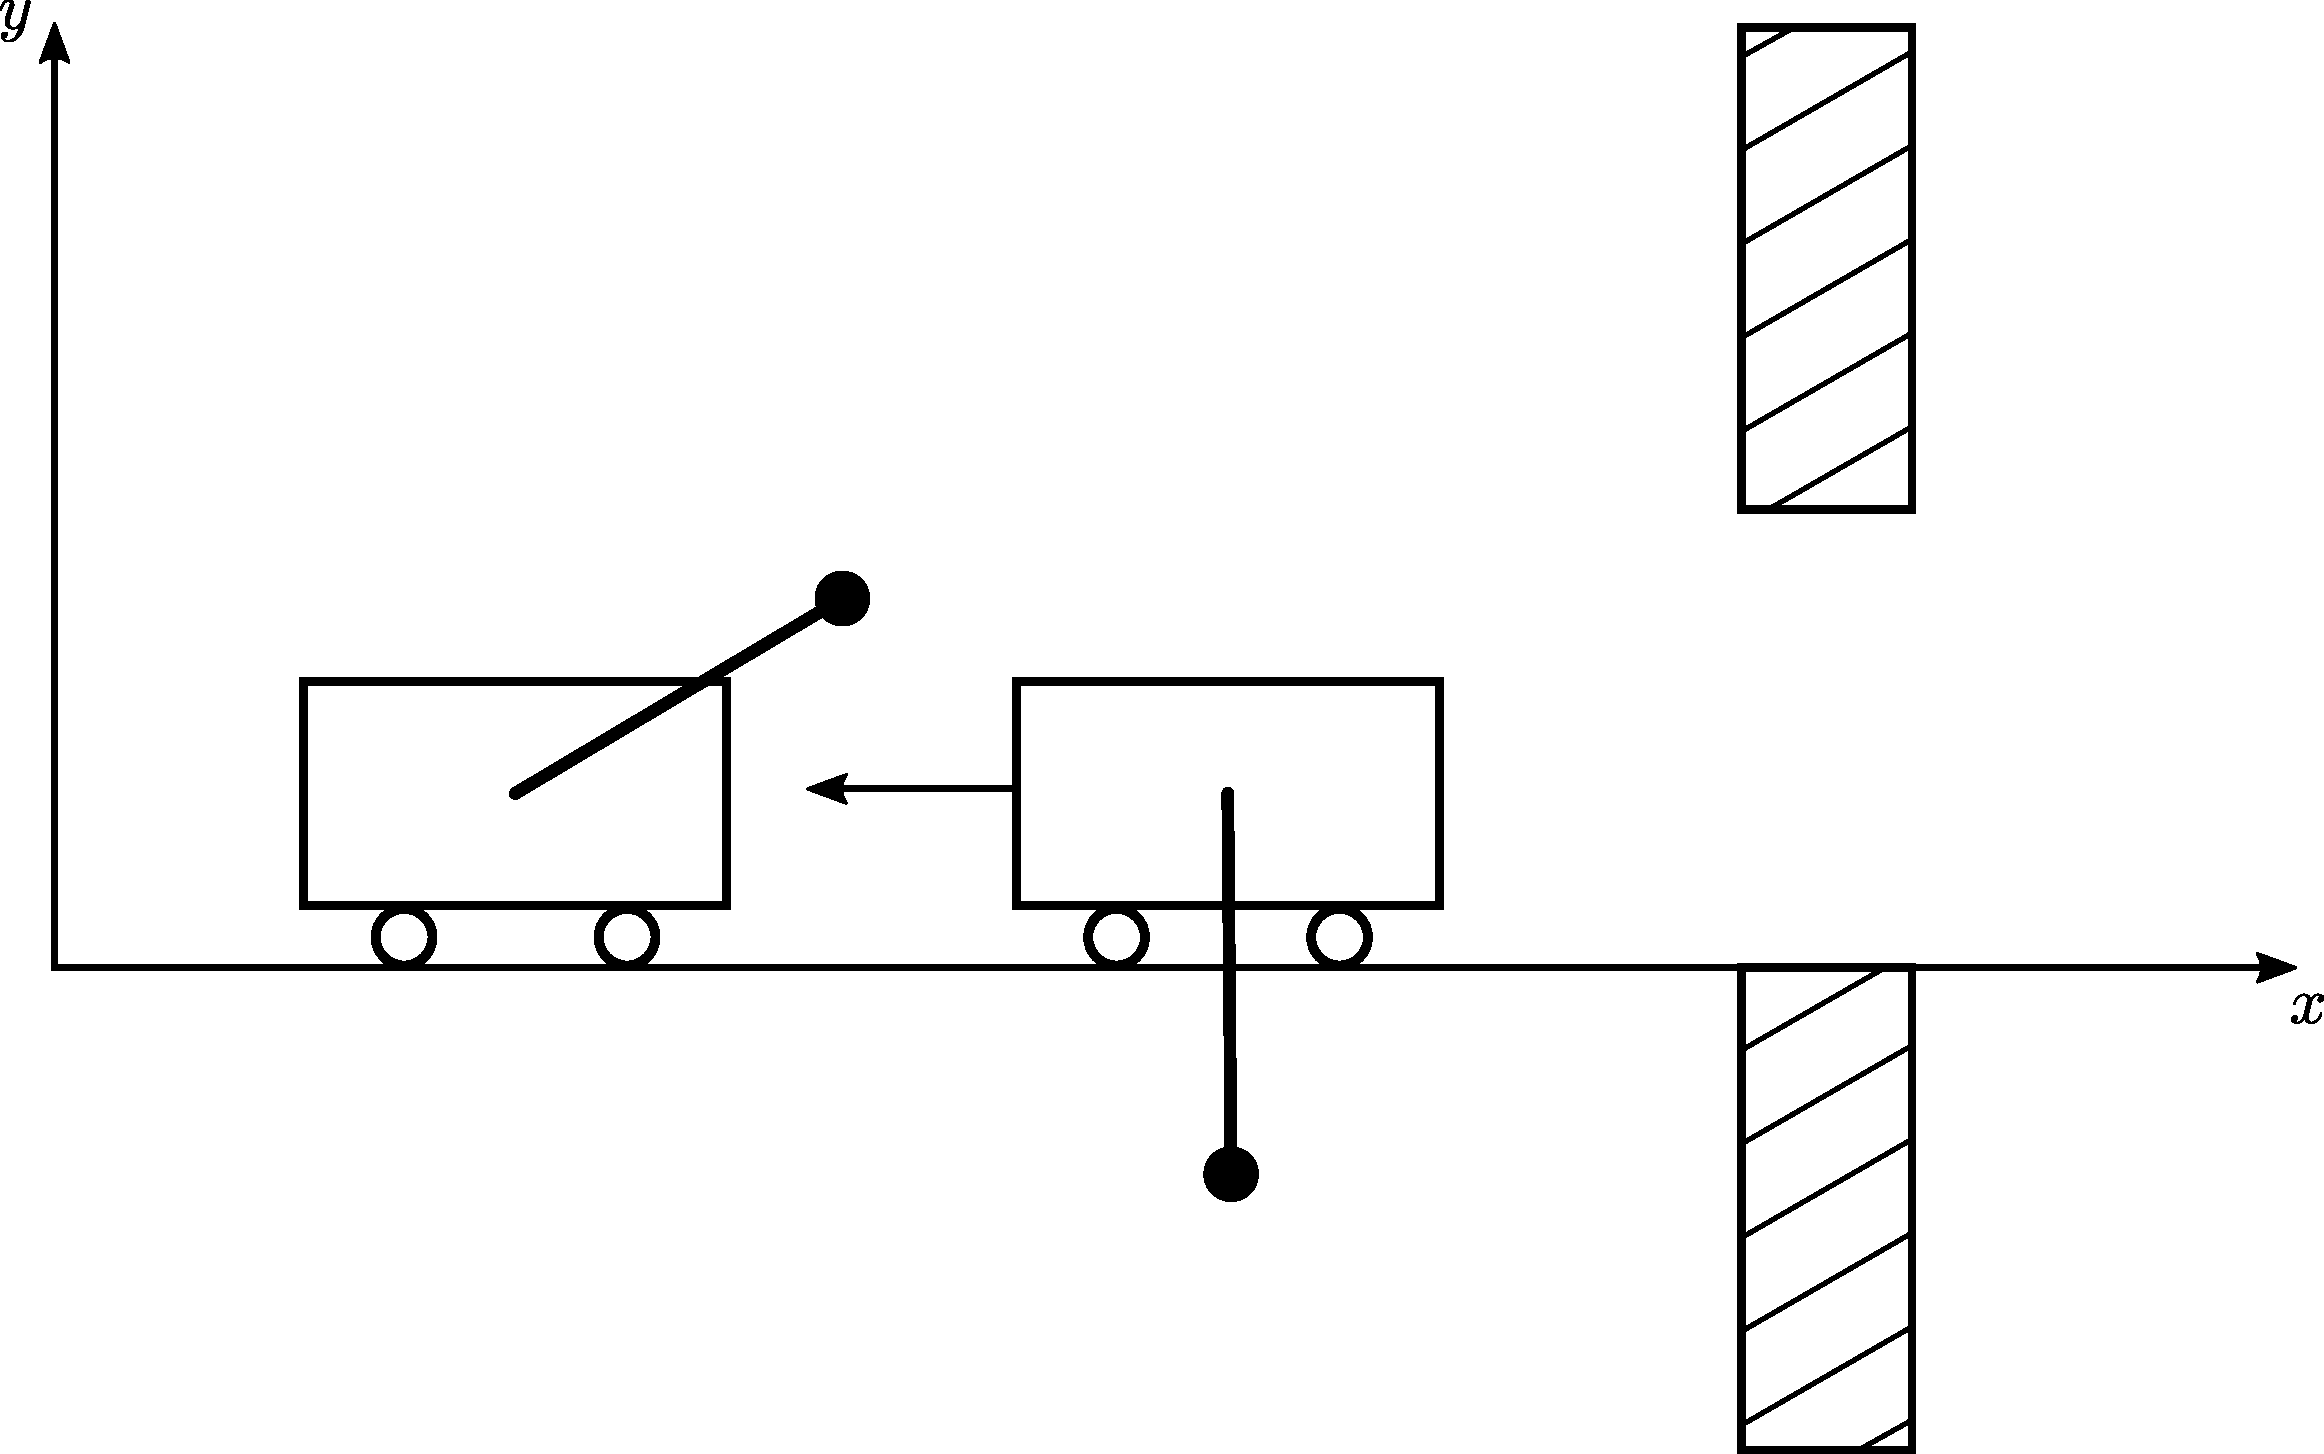
\includegraphics[width=.5\textwidth]{figures/firstTask}
  \caption{The first task is to find a trajectory which raises the pendulum to a position where it is clear of the obstacles in the horizontal direction. Further, to maintain clearance, the angular velocity should hit zero as the target angle is achieved.}
  \label{fig:firstTask}
\end{figure}

The phase portrait in \autoref{fig:phasePortrait}, showing the natural theta-dynamics, it is possible to get an idea of how the pendulum moves. The starting position would be the right-most equilibrium of the phase portrait. If this task should be achieved without external force, the pendulum would have to be initialized in the orbit containing the desired final values. However, by exerting a force on the cart it is possible to shift the theta-dynamics. This is further investigated in the following section.

Assuming that the pendulum was raised above $\frac{\pi}{2}$ while briefly achieving zero angular velocity, the next task would be to maintain zero angular velocity while moving the cart, passing the pendulum through the obstacles, see \autoref{fig:secondTask}.

\begin{figure}[H]
  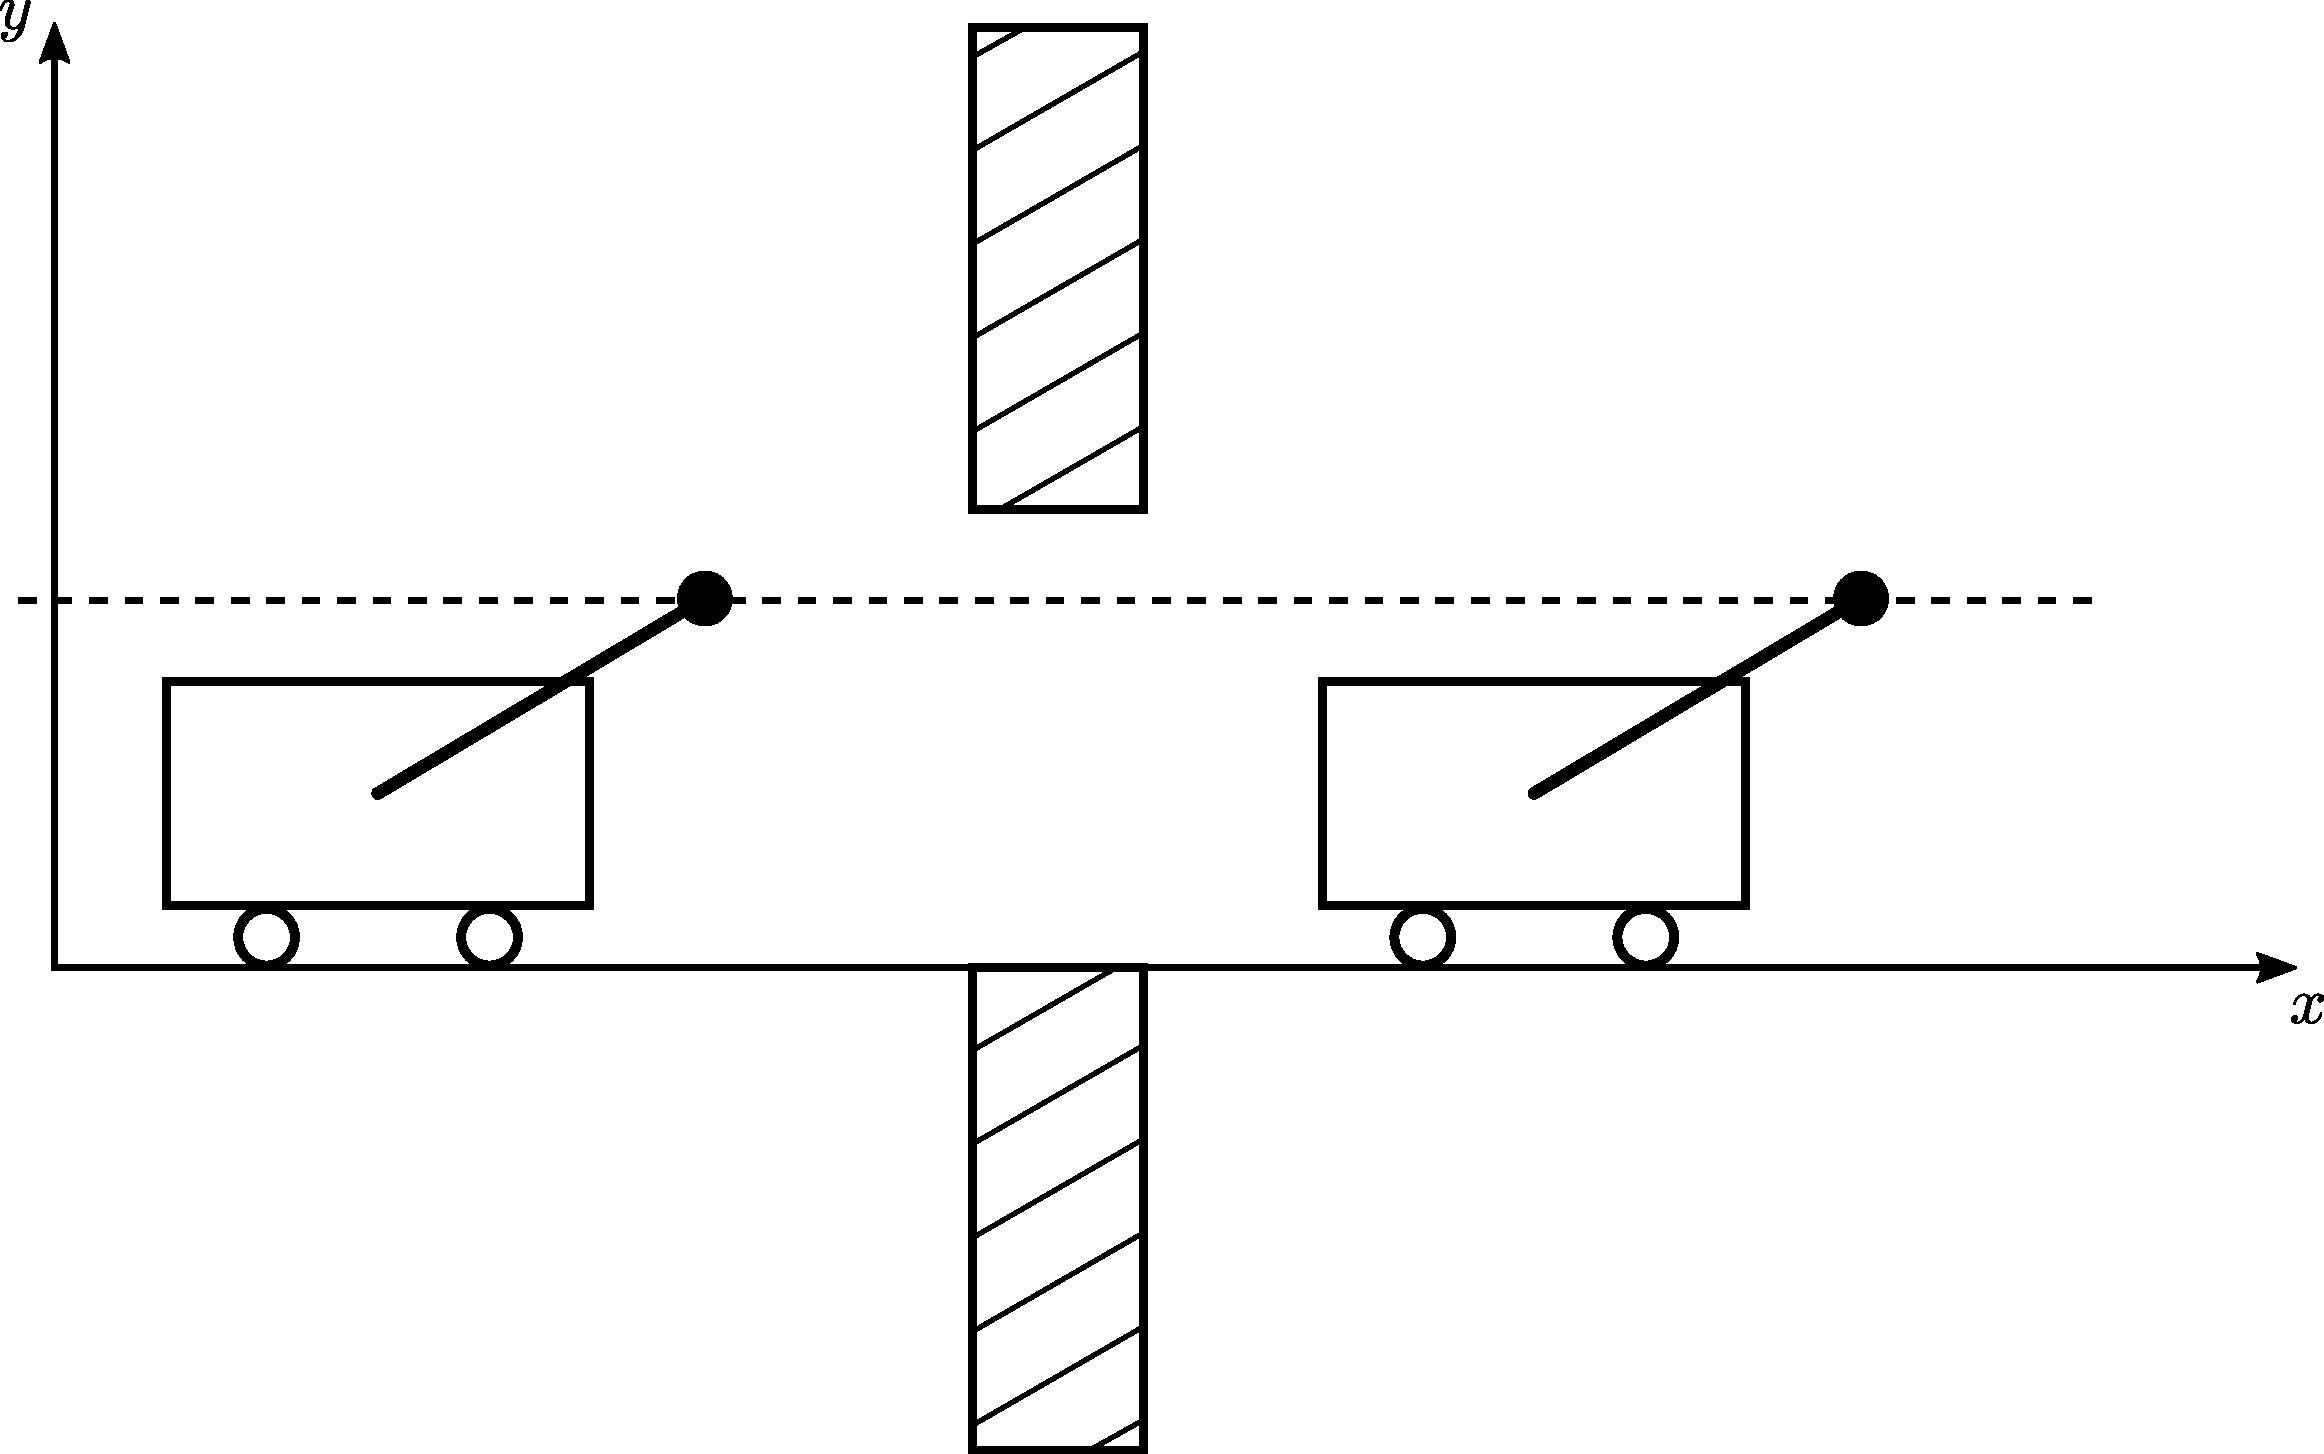
\includegraphics[width=.5\textwidth]{figures/secondTask}
  \caption{The second task is to find a trajectory which keeps the angle and angular velocity at zero as the pendulum is moved with the cart through the obstacles. This can be seen as a virtual constraint where the pendulum is mass is constrained to the dotted line.}
  \label{fig:secondTask}
\end{figure}

Ideally this trajectory is a straight horizontal line. This can be seen as a virtual constraint that forces the angle and the angular velocity to stay unchanged. The result will be significantly reduced dynamics, which can be used to directly achieve the desired trajectory.

Finally it is necessary to recover the system on the other side of the obstacles. It is found that this can be achieved, to some extend, by reversing the first trajectory.
\section{First Trajectory}
Firstly the initial and final values of of $\theta$ and $\dot{\theta}$ are known. Further, the $\theta$-dynamics are known, also for non-zero forces. In the state space and general equations, \autoref{eq:stateSpaceThetaDynamics} and \autoref{eq:alphaBetaGammaGeneral}, the input force is contained by the $\gamma$-function.\\
If now \autoref{eq:alphaBetaGammaGeneral} is seen as an initial value problem. After some manipulation, \fxnote{source Anton's paper(s)} \fxnote{maybe include further explanation/derivations} it is seen that the following function preserves its zero value along the trajectory from initial to final value, assuming the solution exists while requiring $\alpha$ to be non-zero,
%
\begin{flalign}
  \dot{\theta}^2 - \psi (\theta_0, \theta)
  \left(
  \dot{\theta}_0^2 - \int\limits_{\theta_0}^{\theta} \psi (\theta_0, \theta)
  \frac{2 \gamma(s) }{ \alpha(s) } ds
  \right)
  &=  0   \ \ \ , & %\unit{N \cdot m}
  \label{eq:ipv}
\end{flalign}
\ \ \  where,
\begin{flalign}
  \ \ \ \ \ \ \ \psi (\theta_0, \theta) &=
  \exp \left\{
         -2 \int\limits_{\theta_0}^{\theta} \frac{\beta(\tau)}{\alpha(\tau)}  d\tau
       \right\}   \ \ \ . \nonumber &
\end{flalign}

It turns out, that in this case the problem can be solved analytically, and by requiring the final value of the angular velocity be zero, it boils down to,
%
\begin{flalign}
  \left[ -f \frac{m l}{M + m} \sin(s) - m g l \cos(s) \right ]_{\theta_0}^\theta &=  0   \ \ \ . & %\unit{N \cdot m}
  \label{eq:solution}
\end{flalign}

Inserting initial and final value of $\theta$ and solving for f, the force which creates the desired trajectory is obtained. Also note that for this trajectory the applied force is constant and negative, pulling the cart to the left.

Going back to the $\theta$-dynamics, it is possible to construct a phase portrait, see \autoref{fig:phasePortraitFirstTrajectry}, including this negative constant force.

\begin{figure}[H]
  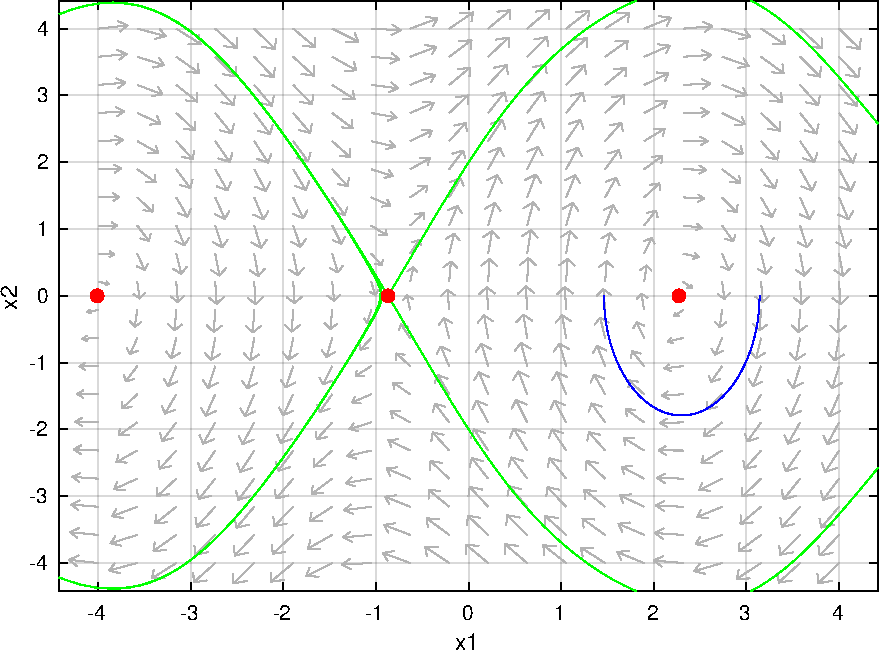
\includegraphics[width=.8\textwidth]{figures/firstTrajectory}
  \caption{Phase portrait of the $\theta$-dynamics including a constant applied force, where $x_1 = \theta$ and $x_2 = \dot{\theta}$. The phase portrait is shifted negatively along $\theta$ because of the applied force. This allows the desired trajectory (blue) from the initial downward position.}
  \label{fig:phasePortraitFirstTrajectry}
\end{figure}

Note how the entire phase portrait is shifted in the negative $\theta$ ($x_1$) direction. This could be expected from \autoref{eq:alphaBetaGamma}, since the force only scales the magnitude of a term which otherwise only depends on $\theta$. Further, the constant force applied is negative, thus the negative shift in the $\theta$ direction.\\
This shift of the phase portrait means that the initial downward position of the pendulum now is placed in an orbit rather than an equilibrium.\\
Additionally, the trajectory (blue) reaches zero angular velocity just as it hits the target angle. The trajectory does however not stop there. It oscillates around the new center equilibrium. Therefore the next input force for the next trajectory must be applied the moment zero angular velocity is achieved.
\section{Second Trajectory}
The second trajectory to complete the task seen in \autoref{fig:secondTask} is different that the first, in that it does not require movement in the ($\theta$, $\dot{\theta}$)-plane, in fact, rather the contrary. It does however require the cart to move forward in order to pass the obstacles and hold up the pendulum.\\
As before, the initial values are known and a final position of the cart can be chosen, which will be the condition for switching to the final task.\\
Substituting the initial values, $\theta = \theta_t$ (target angle), $\dot{\theta} = 0$ and $\ddot{\theta} = 0$, into the dynamic equations, \autoref{eq:dynamicEquation1} and \autoref{eq:dynamicEquation1}, reduces to,
%
\begin{flalign}
  m l \cos \theta_t \ \ddot{x} - m l g \sin \theta_t &=  0  & %\unit{N \cdot m}  \\
  \label{eq:dynamicEquation1SecondTrajectory} \\
  (M+m) \ddot{x} &=  f  \ \ \ . & %\unit{N \cdot m}
  \label{eq:dynamicEquation2SecondTrajectory}
\end{flalign}

In \autoref{eq:dynamicEquation2SecondTrajectory} the force, $f$, is directly provided as a function of the acceleration of the cart. Feeding back $\ddot{x}$ in this manner will attempt to keep the angle of the pendulum steady while moving forward through the obstacles.\\
It is interesting to note that the average of the force excreted during this second trajectory changes the $\theta$-dynamics in such a way that the angle and angular velocity are kept in a saddle point equilibrium.

\begin{figure}[H]
  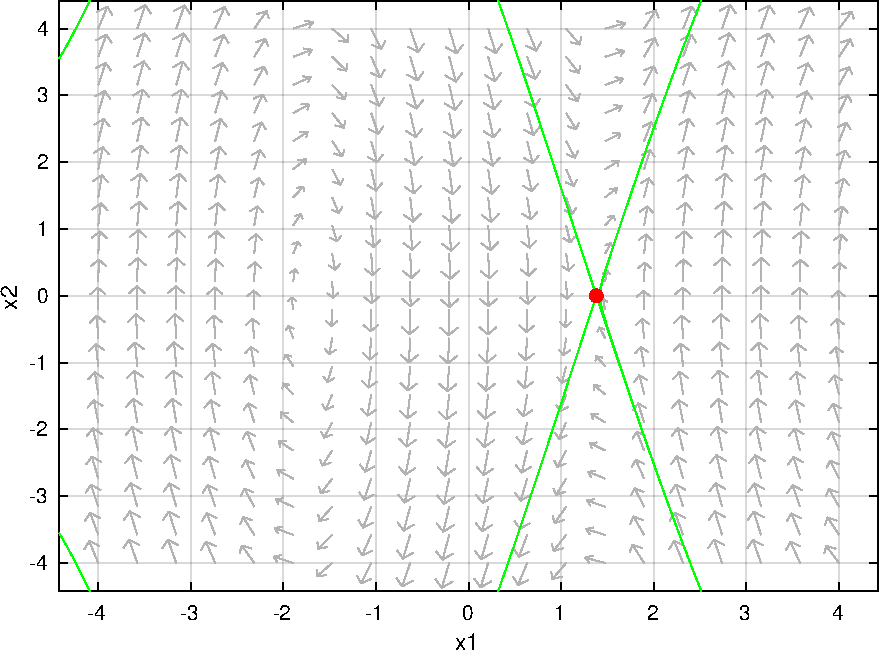
\includegraphics[width=.6\textwidth]{figures/secondTrajectory}
  \caption{Phase portrait showing how the $\theta$-dynamics changes given a constant force averaged from the forces used during the second trajectory. The system is kept near the indicated saddle point equilibrium.}
  \label{fig:phasePortraitSecondTrajectory}
\end{figure}
%\section{Third Trajectory}






%---------- Chapter 3 ----------------------------------------
%\chapter{Chapter 3}

%%% PART 2 %%%
%\part{Design \& Implementation}
%---------- Chapter 4 ---------------------------------------- Modelling
%\chapter{Chapter 4}

%---------- Chapter 5 ---------------------------------------- Control
%\chapter{Chapter 5}

%%% PART 3 %%%
%\part{Test \& Conclusion}
%\chapter{Acceptance Test}
%\chapter{Conclusion}
%\chapter{Discussion}

%%% Setup for Appendix and Bibliography %%%
\bookmarksetup{startatroot}
\addtocontents{toc}{\bigskip}
\newpage
\fancyhead[RO]{\color{aaublue}\small Appendix \nouppercase\rightmark} %even page - chapter title
\fancyhead[LE]{\color{aaublue}\small Appendix \nouppercase\rightmark} %uneven page - section title
\fancyhead[RE,LO]{}
\titleformat{\section}[hang]{\Large\bfseries}{\thesection\hsp\textcolor{aaublue}{|}\hsp}{0pt}{\Large\bfseries}
\renewcommand{\thesection}{\Alph{section}}
\setcounter{section}{0}

%%% APPENDIX %%%
%%%%%%%%%%%%%%%%%%%%%%%%%%%%%%%%%%%%%%%%%\part*{Appendix}

%\addcontentsline{toc}{chapter}{Appendix}

%---------- Appendix A ---------------------------------------- Test Title
%\chapter{Test}

%---------- Appendix B ---------------------------------------- Test Title
%\chapter{Test}

%----------Appendix C ---------------------------------------- Test Title
%\chapter{Test}

%---------- Appendix D ---------------------------------------- Test Title
%\chapter{Test}

%%% BIBLIOGRAPHY %%%
\printbibliography

%%% LIST OF CORRECTIONS %%%
\listoffixmes

\end{document}
